\phantomsection
\addcontentsline{toc}{subsection}{Unidad 2. Oxidación-Reducción}
\subsection*{\textcolor{blueunam}{Unidad 2. Oxidación-Reducción}}

\phantomsection
\addcontentsline{toc}{subsubsection}{Clase 10 -- 29/09/2026: Estados de oxidación en compuestos orgánicos}
\subsubsection*{\textcolor{blueunam}{Clase 10 -- 29/09/2026: Estados de oxidación en compuestos orgánicos}}

\textbf{Número de oxidación (n.o.):} conteo formal que finge que los electrones 
del enlace se los lleva \textbf{completamente} el átomo más electronegativo 
(reparto 100/0). No es una carga real ni un promedio: es una asignación contable 
para rastrear electrones en reacciones redox.

\textbf{Cómo se calcula el n.o. del carbono:} se cuenta la contribución de cada 
enlace del C.

\begin{center}
\begin{tabular}{|l|c|}
\hline
\textbf{Enlace del C} & \textbf{Contribución al n.o.} \\
\hline
A un átomo más electronegativo (O, N, halógeno), enlace simple & $+1$ \\
A un átomo más electronegativo, enlace doble (C=O) & $+2$ \\
A un átomo más electronegativo, enlace triple (C$\equiv$N) & $+3$ \\
A un átomo menos electronegativo (H) & $-1$ \\
A otro C (simple, doble o triple) & $0$ \\
\hline
\end{tabular}
\end{center}

La suma de contribuciones da el n.o. del carbono. En química orgánica estándar 
va de $-4$ a $+4$, con todos los enteros intermedios.

\begin{center}
\begin{tabular}{lccc}
\hline
\textbf{Compuesto} & \textbf{Enlaces del C} & \textbf{n.o. del C} \\
\hline
\ce{CH4}          & 4 C--H                        & $-4$ \\
\ce{CH3-CH3}      & 3 C--H, 1 C--C                & $-3$ \\
\ce{CH3OH}        & 3 C--H, 1 C--O                & $-2$ \\
\ce{CH3-CH2OH}    & 2 C--H, 1 C--C, 1 C--O        & $-1$ \\
\ce{CH2O}         & 2 C--H, 1 C=O                 & $0$  \\
\ce{CH3-CHO}      & 1 C--H, 1 C--C, 1 C=O         & $+1$ \\
\ce{HCOOH}        & 1 C--H, 1 C=O, 1 C--O         & $+2$ \\
\ce{CH3-COOH}     & 1 C--C, 1 C=O, 1 C--O         & $+3$ \\
\ce{CO2}          & 2 C=O                         & $+4$ \\
\hline
\end{tabular}
\end{center}
(Esta tabla y cómo calcular sus n.o. se desarrolla mejor más adelante.) \\

{\small\itshape Nota: en \ce{CH3-CH2OH}, \ce{CH3-CHO} y \ce{CH3-COOH}, el n.o. 
indicado corresponde al carbono señalado (el que tiene el grupo funcional), 
no al \ce{CH3} terminal.}

\textbf{Oxidación:} pérdida de \ce{e^{\color{anblue}-}}. En química orgánica, 
se reduce a ganancia de oxígeno \ce{O} o halógenos, o pérdida de hidrógenos \ce{H}. \\

\textbf{Reducción:} ganancia de \ce{e^{\color{anblue}-}}. En química orgánica, 
se reduce a pérdida de oxígeno \ce{O} o halógenos, o ganancia de hidrógenos \ce{H}.

\begin{notafija}
En toda reacción redox ocurren simultáneamente una oxidación y una reducción. Una no existe sin la otra. Sin embargo, es común nombrar la reacción solo por el proceso que interesa estudiar: ``oxidación del etanol'' aunque el dicromato también se reduce, o ``reducción de la benzofenona'' aunque el 2-propanol también se oxida. Esta convención aparecerá de nuevo cuando se estudien reacciones específicas y en los ejercicios, donde a veces solo se pide analizar una de las dos partes. El nombre no implica que la otra no ocurra.
\end{notafija}

\begin{notaimportante}
\textbf{La notación de transferencia en las flechas.} A lo largo de estos apuntes verás anotaciones como $-2\ce{e-}$, $+2\ce{e-}$, $-\ce{H2O}$ o $+\ce{H2O}$ sobre o debajo de las flechas de reacción. Esta es una convención muy útil que indica el cambio neto que sufre \textbf{nuestra molécula de interés}:
\begin{itemize}
    \item \textbf{Signo negativo ($-\ce{e-}$):} la molécula de interés \textbf{pierde} electrones. Es una oxidación.
    \item \textbf{Signo positivo ($+\ce{e-}$):} la molécula de interés \textbf{gana} electrones. Es una reducción.
    \item El mismo criterio aplica para átomos o moléculas completas (ej. $-\ce{H}$, $-\ce{H2O}$), indicando que la molécula de interés los pierde o los gana.
\end{itemize}
Esta notación es clave porque nos ayuda a visualizar el conteo de electrones de un vistazo, a balancear las ecuaciones y a recordar quién se oxida y quién se reduce. Aunque no escribamos explícitamente al agente oxidante o reductor en la flecha, se da por hecho que existe en el medio (el otro lado de la redox). A veces se anota al inicio de la reacción para saber con qué reacciona, pero durante el proceso se suele omitir.
\end{notaimportante}

Generalmente, si el \ce{C} se enlaza con átomos más electronegativos, hablamos de 
oxidación. Si se enlaza con átomos menos electronegativos, hablamos de reducción. 
(Tomando como referencia el \ce{C}). \\

\textbf{Ejemplos:}
\begin{center}
\begin{tabular}{l@{\qquad}l}
$\ce{Fe^{\color{catred}{2+}}} \longrightarrow \ce{Fe^{\color{catred}{3+}}} + \ce{e^{\color{anblue}-}}$
& (oxidación: perdió 1 \ce{e^{\color{anblue}-}}, carga $+2 \to +3$) \\[8pt]
$\ce{Cu^{\color{catred}{2+}}} + 2\,\ce{e^{\color{anblue}-}} \longrightarrow \ce{Cu}$
& (reducción: ganó 2 \ce{e^{\color{anblue}-}}, carga $+2 \to 0$) \\[8pt]
$\ce{Zn} \longrightarrow \ce{Zn^{\color{catred}{2+}}} + 2\,\ce{e^{\color{anblue}-}}$
& (oxidación: perdió 2 \ce{e^{\color{anblue}-}}, carga $0 \to +2$) \\[8pt]
$\ce{Cl2} + 2\,\ce{e^{\color{anblue}-}} \longrightarrow 2\,\ce{Cl^{\color{anblue}-}}$
& (reducción: ganó 1 \ce{e^{\color{anblue}-}} por átomo, carga $0 \to -1$)
\end{tabular}
\end{center}

\textbf{Aclaración sobre el signo de la carga:} la carga no indica directamente el 
número de electrones, sino el \textbf{balance} entre protones y electrones 
\textbf{respecto al átomo neutro}.

\begin{center}
\begin{tabular}{lcc}
\hline
\textbf{Especie} & \textbf{Carga} & \textbf{Significado} \\
\hline
\ce{Fe^{\color{catred}{3+}}} & $+3$ & 3 protones más que electrones (perdió 3 \ce{e^{\color{anblue}-}} respecto al neutro) \\
\ce{Fe^{\color{catred}{2+}}} & $+2$ & 2 protones más que electrones (perdió 2 \ce{e^{\color{anblue}-}}) \\
\ce{Fe}      & $0$  & Igual número de protones y electrones \\
\ce{Cl^{\color{anblue}-}} & $-1$ & 1 electrón más que protones (ganó 1 \ce{e^{\color{anblue}-}}) \\
\hline
\end{tabular}
\end{center}

Un número más positivo significa \textbf{menos electrones}. Un número más negativo 
significa \textbf{más electrones}. Esto no es intuitivo a primera vista, pero hay 
que recordar que los electrones tienen carga negativa: si el átomo pierde 
electrones (que son negativos), su carga se vuelve más positiva. Por eso $+3$ no 
significa ``3 electrones extra'', sino ``3 electrones de menos''.

\begin{center}
\begin{tikzpicture}[xscale=1.3]
    \draw[-{Stealth}, thick] (-4.8,0) -- (4.8,0);

    \foreach \x in {-4,...,4}
        \draw[thick] (\x,0.18) -- (\x,-0.18);

    \foreach \x in {-4,...,4}
        \node[font=\small, fill=white, inner sep=1.5pt] at (\x,0) {\x};

    \node[left] at (-5.1,0) {\small \textbf{red}};
    \node[right] at (5.1,0) {\small \textbf{oxi}};
\end{tikzpicture}
\end{center}

\textbf{Ejemplos y su posición en la escala:} \\

\textbf{Pasos:}
\begin{enumerate}
    \item Identificar el carbono de interés.
    \item Identificar los sustituyentes directos a su alrededor.
    \item Átomos más electronegativos que el \ce{C}: se les asigna carga 
    $-1$ por cada enlace al carbono, y al carbono se le suma $+1$ por cada 
    enlace con estos.
    \item Átomos menos electronegativos que el \ce{C}: se les asigna carga 
    $+1$ por cada enlace al carbono, y al carbono se le suma $-1$ por cada 
    enlace con estos.
    \item Enlaces \ce{C-C}: aportan $0$ a ambos carbonos.
\end{enumerate} 

\textbf{Nota:} para calcular el n.o. del carbono de interés solo cuentan 
sus enlaces directos. Lo que ocurra con los átomos más allá del primero 
(el \ce{H} de un \ce{O-H}, por ejemplo) no afecta al carbono. Esos enlaces 
solo se consideran cuando se balancea la carga total de la molécula, 
sumando los n.o. de todos los átomos. \\

\textbf{Nota:} en moléculas con varios carbonos con n.o. distinto, 
la escala registra el \textbf{carbono de interés} (el del grupo funcional), 
no un promedio ni la molécula entera. Los demás carbonos tienen su propio 
n.o. que se calcula por separado. \\

\ce{CH4} (Grupo: Alcano) -- Metano: \\
\begin{center}
\schemestart
\chemfig{@{C}C(-[:0]H)(-[:90]H)(-[:180]H)(-[:270]H)}
\schemestop
\chemmove{
    \draw[-{Stealth}, thick] (C) -- +(2,1.5)
        node[right, text width=5cm]{\small El \ce{C} es más electronegativo que el \ce{H}: se lleva los 4\,\ce{e^{\color{anblue}-}}, uno de cada enlace \ce{C-H}};
}
\end{center}
Por lo que para este, el \ce{C} tiene un n.o. de $-4$: \ce{C^{\color{anblue}{4-}}} y cada
\ce{H} tiene n.o. de $+1$: \ce{H^{\color{catred}+}}. En la escala se
posiciona en el estado más reducido: n.o. $= -4$.

\ce{CH3Cl} (Grupo: Haloalcano) -- Clorometano: \\
\begin{center}
\schemestart
\chemfig{C^{\color{anblue}{2-}}(-[:0]Cl^{\color{anblue}-})(-[:90]H^{\color{catred}+})(-[:180]H^{\color{catred}+})(-[:270]H^{\color{catred}+})}
\schemestop
\end{center}
Verificación: $(-2) + 3(+1) + (-1) = 0$. En la escala se posiciona en $-2$.

\ce{CO2} (Grupo: Óxido inorgánico) -- Dióxido de carbono: \\
\begin{center}
\schemestart
\chemfig{C^{\color{catred}{4+}}(=[:0]O^{\color{anblue}{2-}})(=[:180]O^{\color{anblue}{2-}})}
\schemestop
\end{center}
Cada enlace del \ce{C} con un átomo más electronegativo le aporta $+1$ al 
carbono y $-1$ al otro átomo. En el \ce{CO2} cada \ce{O} tiene un enlace 
doble con el \ce{C}, es decir dos enlaces: $2(-1) = -2$, y el \ce{C} queda 
en $+4$. Verificación: $(+4) + 2(-2) = 0$. En la escala se posiciona en 
el estado más oxidado: n.o. $= +4$.

\ce{HCHO / CH2O} (Grupo: Aldehído) -- Metanal / Formaldehído: \\
\begin{center}
\schemestart
\chemfig{C^0(=[:90]O^{\color{anblue}2-})(-[:230]H^{\color{catred}+})(-[:310]H^{\color{catred}+})}
\schemestop
\end{center}
Verificación: $(0) + 2(+1) + (-2) = 0$. En la escala se posiciona en $0$.

\ce{CH2=CH2 / C2H4} (Grupo: Alqueno) -- Eteno / Etileno: \\
\begin{center}
\schemestart
\chemfig{C^{\color{anblue}{2-}}(-[:140]H^{\color{catred}+})(-[:230]H^{\color{catred}+})=C^{\color{anblue}{2-}}(-[:40]H^{\color{catred}+})(-[:320]H^{\color{catred}+})}
\schemestop
\end{center}
Verificación: $2(-2) + 4(+1) = 0$. En la escala se posiciona en $-2$.

\ce{CH3OH / CH4O} (Grupo: Alcohol) -- Metanol / Alcohol metílico: \\
\begin{center}
\schemestart
\chemfig{C^{\color{anblue}{2-}}(-[:0]O^{\color{anblue}{2-}}H^{\color{catred}+})(-[:90]H^{\color{catred}+})(-[:180]H^{\color{catred}+})(-[:270]H^{\color{catred}+})}
\schemestop
\end{center}
Verificación: $(-2) + 4(+1) + (-2) = 0$. En la escala se posiciona en $-2$.

\ce{HCOOH / CH2O2} (Grupo: Ácido carboxílico) -- Ácido metanoico / Ácido fórmico: \\
\begin{center}
\schemestart
\chemfig{C^{\color{catred}{2+}}(=[:90]O^{\color{anblue}2-})(-[:180]H^{\color{catred}+})(-[:0]O^{\color{anblue}2-}(-[:0]H^{\color{catred}+}))}
\schemestop
\end{center}
Verificación: $(+2) + 2(+1) + 2(-2) = 0$. En la escala se posiciona en $+2$.

\ce{HCN} (Grupo: Nitrilo) -- Formonitrilo: \\
\begin{center}
\schemestart
\chemfig{C^{\color{catred}{2+}}(-[:180]H^{\color{catred}+})(~[:0]N^{\color{anblue}{3-}})}
\schemestop
\end{center}
Cada enlace del \ce{C} con un átomo más electronegativo le aporta $+1$ al 
carbono y $-1$ al otro átomo. El \ce{N} tiene un enlace triple con el \ce{C}, 
es decir tres enlaces: $3(-1) = -3$. El \ce{H} es menos electronegativo que 
el \ce{C}, así que el enlace C--H aporta $-1$ al \ce{C} y $+1$ al \ce{H}. 
Sumando: el \ce{C} queda en $+3 - 1 = +2$. Verificación: 
$(+2) + (-3) + (+1) = 0$. En la escala se posiciona en el estado 
$+2$.

\ce{CH3CH2OCH2CH3 / C4H10O} (Grupo: Éter) -- Etoxietano / Dietil éter: \\
\begin{center}
\schemestart
\chemfig{[:-30]-[:30]-O-[:30]-[:-30]}
\qquad\qquad
\chemfig{
[:-30]C^{\color{anblue}{3-}}(-[:140]H^{\color{catred}+})(-[:220]H^{\color{catred}+})(-[:310]H^{\color{catred}+})
-[:30]C^{\color{anblue}{-}}(-[:90]H^{\color{catred}+})(-[:270]H^{\color{catred}+})
-O^{\color{anblue}{2-}}
-[:30]C^{\color{anblue}{-}}(-[:90]H^{\color{catred}+})(-[:270]H^{\color{catred}+})
-[:-30]C^{\color{anblue}{3-}}(-[:40]H^{\color{catred}+})(-[:230]H^{\color{catred}+})(-[:310]H^{\color{catred}+})
}
\schemestop
\end{center}
Verificación: $2(-3) + 2(-1) + (-2) + 10(+1) = 0$. En la escala se posiciona en $-1$ (C unido al \ce{O}). \\
\textbf{Nota:} los enlaces C--C no aportan carga (paso 5), por eso cada 
carbono puede tener n.o. distinto dentro de la misma molécula. Conviene 
distinguir entre el n.o. de un carbono individual y la suma de todos los 
n.o., que en una molécula neutra da $0$. Además existe otro concepto: la 
suma de las cargas de todos los carbonos, que indica cuánta carga aportan 
los demás átomos para balancear. Ese segundo concepto se desarrolla 
más adelante.

\ce{CCl4} (Grupo: Haloalcano) -- Tetraclorometano: \\
\begin{center}
\schemestart
\chemfig{C^{\color{catred}{4+}}(-[:0]Cl^{\color{anblue}-})(-[:90]Cl^{\color{anblue}-})(-[:180]Cl^{\color{anblue}-})(-[:270]Cl^{\color{anblue}-})}
\schemestop
\end{center}
Verificación: $(+4) + 4(-1) = 0$. En la escala se posiciona en $+4$.

\ce{CH3COCH3 / C3H6O} (Grupo: Cetona) -- Propanona / Acetona: \\
\begin{center}
\schemestart
\chemfig{C^{\color{catred}{2+}}(=[:90]O^{\color{anblue}{2-}})(-[:225]^{\color{anblue}{3-}})(-[:315]^{\color{anblue}{3-}})}
\schemestop
\end{center}
Verificación: $(+2) + 2(-3) + (-2) + 6(+1) = 0$. En la escala se posiciona en $+2$.

\ce{C6H12} (Grupo: Cicloalcano) -- Ciclohexano: \\
\begin{center}
\schemestart
\chemfig{*6(^{\color{anblue}{2-}}-^{\color{anblue}{2-}}-^{\color{anblue}{2-}}-^{\color{anblue}{2-}}-^{\color{anblue}{2-}}-^{\color{anblue}{2-}}-)}
\schemestop
\end{center}
Verificación: $6(-2) + 12(+1) = 0$. En la escala se posiciona en $-2$.

\ce{C6H6} (Grupo: Areno) -- Benceno: \\
\begin{center}
\schemestart
\chemfig{*6(^{\color{anblue}{-}}=^{\color{anblue}{-}}-^{\color{anblue}{-}}=^{\color{anblue}{-}}-^{\color{anblue}{-}}=^{\color{anblue}{-}}-)}
\schemestop
\end{center}
Verificación: $6(-1) + 6(+1) = 0$. En la escala se posiciona en $-1$.

\begin{center}
\begin{tikzpicture}[xscale=1.5, yscale=1.5]
    \draw[-{Stealth}, thick] (-4.2,0) -- (4.2,0);

    \foreach \x in {-4,...,4}
        \draw[thick] (\x,0.15) -- (\x,-0.15);

    \foreach \x in {-4,...,4}
        \node[font=\small, fill=white, inner sep=1.5pt] at (\x,0) {\x};

    \node[left] at (-4.5,0) {\small \textbf{red}};
    \node[right] at (4.5,0) {\small \textbf{oxi}};

    % -4
    \node[above=10pt] at (-4,0) {\small \ce{CH4}};

    % -2 (cuatro compuestos apilados)
    \node[above=10pt] at (-2,0) {\small \ce{CH3OH}};
    \node[above=28pt] at (-2,0) {\small \ce{CH3Cl}};
    \node[below=10pt] at (-2,0) {\small \ce{C2H4}};
    \node[below=28pt] at (-2,0) {\small \ce{C6H12}};

    % -1
    \node[above=10pt] at (-1,0) {\small \ce{C6H6}};
    \node[below=10pt] at (-1,0) {\small éter};

    % 0
    \node[above=10pt] at (0,0) {\small \ce{HCHO}};

    % +2 (tres compuestos apilados)
    \node[above=10pt] at (2,0) {\small \ce{HCOOH}};
    \node[below=10pt] at (2,0) {\small \ce{HCN}};
    \node[below=28pt] at (2,0) {\small Acetona};

    % +4
    \node[above=10pt] at (4,0) {\small \ce{CO2}};
    \node[below=10pt] at (4,0) {\small \ce{CCl4}};
\end{tikzpicture}
\end{center}

Una vez vistos varios ejemplos se pueden notar dos cosas. Imaginemos la 
reacción de combustión del metano:

\begin{center}
\schemestart
\ce{CH4}
\+
\ce{2O2}
\arrow{->[$\Delta$][$-8\ce{e-}$]}
\ce{CO2}
\+
\ce{2H2O}
\schemestop
\end{center}

Es un proceso de oxidación del \ce{C^{\color{anblue}{4-}}} al 
\ce{C^{\color{catred}{4+}}}, con un cambio neto de 8 electrones en un solo 
paso. Sin embargo, esto no significa que todas las oxidaciones sean así. 
La serie de compuestos que va del metano al dióxido de carbono muestra que 
la oxidación del carbono puede darse en saltos de 2 electrones cuando el 
proceso se controla paso a paso:

\begin{center}
\schemestart
\ce{CH4}
\arrow{->[$-2\ce{e-}$]}
\ce{CH3OH}
\arrow{->[$-2\ce{e-}$]}
\ce{CH2O}
\arrow{->[$-2\ce{e-}$]}
\ce{HCOOH}
\arrow{->[$-2\ce{e-}$]}
\ce{CO2}
\schemestop
\\[8pt]
{\small $n.o.$: \quad $-4$ \quad $\longrightarrow$ \quad $-2$ \quad 
$\longrightarrow$ \quad $0$ \quad $\longrightarrow$ \quad $+2$ \quad 
$\longrightarrow$ \quad $+4$}
\end{center}

\textbf{Para qué sirve el n.o.:}

\begin{enumerate}
    \item \textbf{Reactividad.} El n.o. indica si el C es pobre o rico en 
    densidad electrónica, y por lo tanto qué lo ataca. Un n.o. alto 
    significa que el C está deficiente de electrones y tiene carga parcial 
    positiva, así que se comporta como electrófilo y lo atacan los 
    nucleófilos. El \ce{CO2}, con su C en $+4$, reacciona con 
    \ce{OH^{\color{anblue}{-}}} para dar bicarbonato. En cambio, un n.o. 
    bajo significa que el C está saturado de electrones y no tiene nada 
    que un nucleófilo quiera atacar. El \ce{CH4}, con su C en $-4$, no 
    reacciona con \ce{OH^{\color{anblue}{-}}}, pero sí con oxidantes como 
    el \ce{O2}, que arrancan electrones de donde sobran. Un n.o. intermedio 
    tiene ambas rutas. El metanal, por ejemplo, puede oxidarse a ácido 
    fórmico o reducirse a metanol según las condiciones. El n.o. da la 
    dirección termodinámica pero no la velocidad. El \ce{CO2} podría 
    reaccionar con agua, pero la barrera de activación es alta y a 
    temperatura ambiente no lo hace.

    \item \textbf{Energía almacenada.} Un enlace fuerte cuesta mucho 
    romperlo, mientras que uno débil cuesta poco. La fuerza viene de la 
    diferencia de electronegatividad entre los átomos. Cuando un átomo muy 
    electronegativo, como el O, atrae los electrones compartidos, el enlace 
    se polariza y gana una estabilización electrostática extra. En cambio, 
    cuando los dos átomos tienen electronegatividad parecida, como C y H o 
    C y C, la compartición es casi equitativa y el enlace queda débil.

    Los enlaces alrededor de un C reducido, \ce{C-H} y \ce{C-C}, son 
    débiles y tienen energías de $\sim$413 y $\sim$347 kJ\,mol$^{-1}$. 
    Los de un C oxidado, \ce{C=O} y \ce{O-H}, son fuertes y tienen 
    $\sim$745 y $\sim$463 kJ\,mol$^{-1}$.

    Al oxidar un compuesto se rompen enlaces débiles y se forman enlaces 
    fuertes. Formar un enlace fuerte libera más energía de la que costó 
    romper uno débil, y esa diferencia sale como calor. Por eso los 
    combustibles son moléculas reducidas como el metano, el octano o la 
    glucosa, mientras que el \ce{CO2} es el producto final inerte de la 
    combustión y la respiración: ya está en el fondo del pozo energético.

    \item \textbf{Reacciones posibles.} El C tiene cuatro electrones de 
    valencia, ni más ni menos. Por eso los n.o. extremos son $+4$ y $-4$. 
    En el \ce{CO2} el carbono perdió los cuatro, y en el \ce{CH4} los 
    ganó. No existen n.o. $+5$ o $-5$ estables. Del $-4$ solo se puede 
    oxidar, porque ya no hay más electrones que ganar. Del $+4$ solo se 
    puede reducir, porque ya no hay más electrones que perder. Del 
    intermedio se pueden hacer ambas. Con esto se predice qué transformación 
    es posible antes de intentar la reacción. Un compuesto en $+3$, como 
    el ácido acético \ce{CH3-COOH}, puede oxidarse a $+4$ o reducirse 
    hacia abajo, pero no puede saltar directo a $-4$ en un solo paso 
    concertado.

    \item \textbf{Equivalencia entre compuestos.} La serie \ce{CH4} 
    ($-4$) $\to$ \ce{CH3OH} ($-2$) $\to$ \ce{CH2O} ($0$) $\to$ \ce{HCOOH} 
    ($+2$) $\to$ \ce{CO2} ($+4$) avanza de 2 en 2 electrones porque ningún 
    compuesto tiene enlaces C--C. Cuando aparecen enlaces C--C, también 
    aparecen valores impares como $-3$, $-1$, $+1$ y $+3$. El n.o. permite 
    comparar dos compuestos cualesquiera de la serie, no solo los vecinos. 
    Por ejemplo, de \ce{CH4} a \ce{HCOOH} se transfieren 6 electrones. Esto 
    sirve para balancear semirreacciones redox o para calcular cuánto 
    oxidante se necesita en una reacción.

    \textbf{Por qué los saltos son de 2 electrones.} Los enlaces covalentes 
    contienen pares de electrones. Cuando un enlace C--H se convierte en 
    C--OH o en C=O, los dos electrones del enlace original se reorganizan 
    para formar el nuevo enlace con el heteroátomo. En esta serie el 
    heteroátomo es siempre el oxígeno, pero la regla es general: también 
    aplica con N, Cl o cualquier átomo más electronegativo que el C. Cada 
    heteroátomo incorporado representa un par de electrones transferidos, 
    y la oxidación avanza de 2 en 2. En las reacciones polares comunes, 
    como la sustitución nucleofílica, la eliminación o la adición a un 
    carbonilo, las flechas curvas siempre representan el movimiento de un 
    par de electrones, nunca de uno solo.

    Los saltos de 1 electrón sí existen, pero generan radicales, especies 
    con un electrón desapareado y de vida corta. Cuando ocurre una 
    transferencia de un solo electrón, la reacción deja de ser polar y se 
    vuelve radicalaria por definición. Esto pasa en la formación de 
    reactivos de Grignard, en la reducción de Birch, en fotoredox y en la 
    combustión, donde las cadenas radicalarias propagan la reacción 
    quitando hidrógenos de a uno. También aparece con metales de transición 
    que cambian de estado de oxidación en una unidad, como el par 
    \ce{Fe^{\color{catred}{2+}}}/\ce{Fe^{\color{catred}{3+}}}, porque el hierro 
    puede ceder o aceptar electrones de uno en uno. En bioquímica, en 
    cambio, la cadena transportadora de electrones mueve los electrones de 
    a pares a través de deshidrogenasas que los transfieren al \ce{NAD+} 
    o al \ce{FAD}, manteniendo la lógica de 2 en 2.
\end{enumerate}

\textbf{Suma de n.o. de todos los carbonos.} Hasta aquí cada cálculo fue 
para un carbono individual, el del grupo funcional. Pero también se puede 
sumar el n.o. de \textbf{todos} los carbonos de la molécula. Esa suma 
indica la carga que aporta el esqueleto carbonado, y el resto de los 
átomos (H, O, N, halógenos) suman lo opuesto para balancear.

\textbf{Regla:} la suma de los n.o. de \emph{todos} los átomos es igual a 
la carga total de la especie. En una molécula neutra da $0$, en un catión 
da la carga positiva, en un anión da la carga negativa.

\textbf{Atajo:} contar los H y los heteroátomos es más rápido que analizar 
cada carbono. Lo que falte para llegar a la carga total es lo que aportan 
los carbonos.

\textbf{Ejemplo 1: isopropanol} \ce{CH3-CH(OH)-CH3}.

\begin{itemize}
    \item 7 \ce{H} unidos a C: $7(+1) = +7$
    \item 1 \ce{O} unido solo al C: $-1$
    \item El \ce{H} del \ce{O-H} no cuenta: junto con el \ce{O} suman $+1 - 1 = 0$
    \item Total H + O: $+6$
    \item Molécula neutra, así que la suma de C debe ser $-6$
\end{itemize}

Verificación por carbono: C1 (CH$_3$) $= -3$, C2 (CH) $= 0$, C3 (CH$_3$) $= -3$. Suma: $-6$.

\textbf{Ejemplo 2: catión alílico} \ce{CH2=CH-CH2+}.

\begin{itemize}
    \item 5 \ce{H} unidos a C: $5(+1) = +5$
    \item Sin heteroátomos
    \item Carga total del ion: $+1$
    \item Suma de C: $-(+5) + (+1) = -4$
\end{itemize}

Verificación por carbono: C1 (CH$_2$=) $= -2$, C2 (CH=) $= -1$, C3 (CH$_2^+$) $= -1$. Suma: $-4$.

\textbf{Utilidad en moléculas grandes.} En una molécula con muchos 
carbonos, calcular el n.o. de cada uno por separado es tedioso. La suma 
total de carbonos se obtiene de una sola cuenta con los H y heteroátomos, 
y comparar esa suma antes y después de una reacción da directamente los 
electrones transferidos. En materiales como los COFs, donde cada nodo 
repite el patrón miles de veces, este atajo es la forma práctica de 
rastrear la carga en la red sin analizar cada carbono individual.

\textbf{Ejemplo de COFs:}
\begin{center}
\schemestart
\chemfig{
    *6((-F)=(
        -N=[:225]-[:270](*6(=-=-=(
            -[:45]\chembelow{N}{H}-[:-45]-[:45](*6(=-=-(
                -[:90]N=[:45]-[:90](*6(=-=-(
                    -[:135]=[:225]N?
                )=-))
            )=-))
        )-))
    )-(-F)=?-(-F)=(-F)-(-F))
}
\schemestop
\end{center}

\textbf{Análisis de n.o. en el fragmento de COF.} El fragmento tiene 
cuatro tipos de carbono distinguibles por sus sustituyentes.

\begin{center}
\small
\renewcommand{\arraystretch}{1.5}
\begin{tabular}{lccc}
\hline
\textbf{Tipo} & \textbf{Enlaces del C} & \textbf{n.o.} & \textbf{Ubicación} \\
\hline
C--F aromático    & 2 C--C, 1 C--F        & $+1$ & anillo fluorado \\
C--H aromático    & 2 C--C, 1 C--H        & $-1$ & anillos externos \\
C=N imina         & 1 C--H, 1 C=N, 1 C--C & $+1$ & enlace \ce{CH=N} \\
CH$_2$ amina      & 2 C--H, 1 C--N, 1 C--C & $-1$ & puente \ce{NH-CH2} \\
\hline
\end{tabular}
\normalsize
\end{center}

\textbf{Cambio por sustitución.} Reemplazar un H aromático por un F 
sube el n.o. de ese carbono de $-1$ a $+1$, un salto de $2$ electrones. 
Es el mismo patrón de la serie \ce{CH4} $\to$ \ce{CO2}, pero aplicado a 
un solo carbono del anillo. En un COF, esto permite modular las 
propiedades electrónicas de un nodo específico sin tocar el resto de la 
red, porque los enlaces C--C (que conectan los nodos entre sí) aportan 
$0$ al n.o. y aíslan el efecto.

\textbf{Suma de carbonos en el fragmento.} Para verificar la coherencia 
del balance, se suman los n.o. de todos los carbonos del fragmento y se 
compara con la carga total, que es $0$ porque la molécula es neutra. El 
resto de los átomos (\ce{H}, \ce{F}, \ce{N}) compensan esa suma:

\begin{center}
\begin{tabular}{lc}
\hline
\textbf{Grupo} & \textbf{Aporte} \\
\hline
Carbonos (suma)   & valor neto \\
Hidrógenos        & $+1$ cada uno \\
Flúor             & $-1$ cada uno \\
Nitrógeno         & $-3$ en imina, $-2$ en amina \\
\hline
Total             & $0$ \\
\hline
\end{tabular}
\end{center}

\textbf{Nota:} el esquema mostrado es un \emph{fragmento modelo}, no un COF 
completo. Un COF real es una red extendida en dos o tres dimensiones donde 
cada nodo se conecta a tres o más vecinos mediante enlaces imina 
(\ce{-CH=N-}), formando una estructura porosa infinita. Aquí se ha cerrado 
el macrociclo para poder mostrarlo como una sola molécula y aplicar el 
análisis de n.o. Los F en los bordes representan sustituyentes que en el 
material real estarían apuntando hacia otros nodos o hacia el espacio 
de poro.

\phantomsection
\addcontentsline{toc}{subsubsection}{Clase 11 -- 01/10/2026: Nivel de oxidación global}
\subsubsection*{\textcolor{blueunam}{Clase 11 -- 01/10/2026: Nivel de oxidación global}}

Además del n.o. de un carbono individual, se puede asignar un 
\textbf{nivel de oxidación global} a una molécula completa. Este número 
caracteriza el estado redox de la molécula entera y sirve para rastrear 
cambios globales en una transformación, no de un sitio específico.

\textbf{Heteroátomo:} átomo distinto de C e H dentro de una molécula 
orgánica. Los más comunes son \ce{O}, \ce{N}, \ce{S} y los halógenos 
(\ce{F}, \ce{Cl}, \ce{Br}, \ce{I}). Introducen diferencia de 
electronegatividad en el esqueleto carbonado, y cada uno cuenta como $+1$ 
en la fórmula.

\textbf{Fórmula general:}
\begin{equation}
\text{n.o. global} = \text{heteroátomos} + \text{anillos} + \text{enlaces } \pi
\end{equation}

\textbf{Cómo se cuenta cada término:}
\begin{itemize}
    \item \textbf{Heteroátomos:} número total de heteroátomos presentes.
    \item \textbf{Anillos:} número de anillos en la molécula.
    \item \textbf{Enlaces $\pi$:} número de dobles enlaces. Los aromáticos cuentan sus dobles individuales.
\end{itemize}

\textbf{Interpretación:}
\begin{itemize}
    \item Un n.o. global \textbf{más bajo} indica una molécula más reducida.
    \item Un n.o. global \textbf{más alto} indica una molécula más oxidada.
    \item Si en una transformación el n.o. global \textbf{no cambia}, el proceso 
    es intramolecular (reorganización interna) y no hay redox neto.
    \item Si el n.o. global \textbf{cambia}, hay redox. La magnitud del cambio 
    indica cuántos electrones se transfieren y si la conversión puede darse 
    en un solo paso o requiere intermediarios (radicales, carbocationes, etc.).
\end{itemize}

\textbf{Ejemplo.} La molécula \chemfig{*6(=-=(-=[:-30])-=-)} (ciclohexadieno 
con sustituyente vinilo) tiene:
\begin{itemize}
    \item Heteroátomos: $0$
    \item Anillos: $1$
    \item Enlaces $\pi$: $4$ (tres del anillo aromático y uno del vinilo)
\end{itemize}
\[
\text{n.o. global} = 0 + 1 + 4 = 5
\]

Al comparar con otra molécula o con el producto de una transformación, la 
diferencia entre los dos n.o. globales da directamente los electrones 
transferidos en el proceso global.

\textbf{Ejemplo.} Pinacol $\to$ pinacolona. \\

\begin{center}
\schemestart
\chemname{\chemfig{CH_3-C^{\color{catred}{+}}(-[:90]OH)(-[:270]CH_3)-C^{\color{catred}{+}}(-[:90]CH_3)(-[:0]OH)(-[:270]CH_3)}}{2,3-dimetil-2,3-butanodiol}
\arrow{->}
\chemname{\chemfig{CH_3-C^0(-[:90]CH_3)(-[:270]CH_3)-C^{\color{catred}{2+}}(-[:90]CH_3)(=[:270]O)}}{3,3-dimetil-2-butanona}
\schemestop
\end{center}

\begin{center}
\renewcommand{\arraystretch}{1.4}
\begin{tabular}{lcccc}
\hline
\textbf{Molécula} & \textbf{Heteroátomos} & \textbf{Anillos} & \textbf{Enlaces }$\boldsymbol{\pi}$ & \textbf{n.o. global} \\
\hline
Pinacol    & $2$ (\ce{O}) & $0$ & $0$ & $2$ \\
Pinacolona & $1$ (\ce{O}) & $0$ & $1$ (\ce{C=O}) & $2$ \\
\hline
\end{tabular}
\end{center}

El n.o. global es igual en reactivo y producto, así que la transformación 
no es redox neta: es una reorganización intramolecular.

\textbf{Ejemplo.} Fotoreducción de benzofenona con 2-propanol. \\

Benzofenona + 2-propanol $\longrightarrow$ Benzopinacol + Propanona \\[8pt]

\begin{center}
\setchemfig{atom sep=2em}
\chemnameinit{}
\schemestart
2\,\chemname{\chemfig[baseline=(current bounding box.center)]{O=[:270]C^{\color{catred}{+2}}(-[:225]*6(=-=-=-))(-[:-45]*6(=-=-=-))}}{Benzofenona}
\+
\chemname{\chemfig[baseline=(current bounding box.center)]{C^0(-[:90]OH)(-[:-45]CH_3)(-[:225]CH_3)}}{2-propanol}
\arrow{->[$-2\ce{e-}$]}
\chemname{\chemfig[baseline=(current bounding box.center)]{C^{\color{catred}{+1}}(-[:135]*6(=-=-=-))(-[:225]*6(=-=-=-))(-[:270]OH)-C^{\color{catred}{+1}}(-[:45]*6(=-=-=-))(-[:-45]*6(=-=-=-))(-[:90]OH)}}{Benzopinacol}
\+
\chemname{\chemfig[baseline=(current bounding box.center)]{C^{\color{catred}{+2}}(=[:90]O)(-[:-45]CH_3)(-[:225]CH_3)}}{Propanona}
\schemestop
\chemnameinit{}
\end{center}

En esta reacción, la oxidación y la reducción ocurren de manera simultánea 
en un proceso global de dos electrones. El 2-propanol actúa como agente 
reductor, oxidándose a propanona, mientras que la benzofenona se reduce a 
benzopinacol. Dado que se requieren dos moléculas de benzofenona para 
captar los dos electrones (y los hidrógenos) que libera el 2-propanol, 
la transferencia neta es de 2 electrones. El mecanismo real ocurre a 
través de la transferencia de átomos de hidrógeno (vía radicales) desde 
el alcohol hacia la benzofenona excitada por la luz, pero el balance 
global corresponde a una redox de dos electrones.

\textbf{Nombres IUPAC:}
\begin{itemize}
    \item Benzofenona: difenilmetanona
    \item 2-propanol: propan-2-ol
    \item Benzopinacol: 1,1,2,2-tetrafeniletano-1,2-diol
    \item Propanona: propan-2-ona (acetona)
\end{itemize}

\textbf{Balanceo:}
\[
\ce{2 (C6H5)2C=O + (CH3)2CHOH -> (C6H5)2C(OH)-C(OH)(C6H5)2 + (CH3)2C=O}
\]

\textbf{Suma de n.o. global:}
\begin{center}
\renewcommand{\arraystretch}{1.4}
\begin{tabular}{lcccc}
\hline
\textbf{Molécula} & \textbf{Heteroátomos} & \textbf{Anillos} & \textbf{Enlaces }$\boldsymbol{\pi}$ & \textbf{n.o. global} \\
\hline
Benzofenona ($\times 2$) & $2$ & $4$ & $14$ & $20$ \\
2-propanol & $1$ & $0$ & $0$ & $1$ \\
\hline
\textbf{Total reactivos} & & & & $21$ \\
\hline
Benzopinacol & $2$ & $4$ & $12$ & $18$ \\
Propanona & $1$ & $0$ & $1$ & $2$ \\
\hline
\textbf{Total productos} & & & & $20$ \\
\hline
\end{tabular}
\end{center}

Las sumas de n.o. global en reactivos y productos no coinciden exactamente 
($21$ contra $20$). Este desfase de una unidad es un artefacto de cómo 
la fórmula cuenta los enlaces \(\pi\) y los anillos en moléculas que se 
dimerizan (dos moléculas se unen en una); no representa una transferencia 
real de un solo electrón. El balance estequiométrico y el cambio de estados 
de oxidación de los carbonos reactivos confirman que la transferencia neta 
en esta reacción es de \textbf{2 electrones}.

\phantomsection
\addcontentsline{toc}{subsubsection}{Balanceo de reacciones orgánicas (Método del [H])}
\subsubsection*{\textcolor{blueunam}{Balanceo de reacciones orgánicas (Método del [H])}}

En química orgánica, el balanceo de reacciones redox no suele hacerse contando electrones libres, sino utilizando el concepto de \textbf{hidrógeno naciente} o \textbf{[H]}. Este método es una adaptación directa del método del ion-electrón, pero resulta mucho más intuitivo para moléculas con esqueletos carbonados.

\textbf{El equivalente químico:} un \ce{[H]} representa formalmente un protón y un electrón.
\[
\ce{[H] \equiv H+ + e-}
\]
Por lo tanto, transferir dos \ce{[H]} es exactamente lo mismo que transferir dos electrones.

\textbf{Especies espectadoras y herramientas de balanceo.}
Antes de aplicar el método, es crucial identificar a los \textbf{iones espectadores}. En las reacciones redox, iones como el potasio (\ce{K+}) o el sodio (\ce{Na+}) no participan en la transferencia de electrones; su número de oxidación no cambia. Por eso se ignoran en las semirreacciones y se trabajan solo con las especies que sí se oxidan o reducen (como el dicromato, \ce{Cr2O7^{2-}}). Al final, los espectadores vuelven a aparecer para formar las sales.

\textbf{Nota importante:} a diferencia de los iones espectadores, los átomos de hidrógeno y oxígeno \textbf{nunca} se ignoran. El agua (\ce{H2O}), los protones (\ce{H+}) y los hidrógenos nacientes (\ce{[H]}) son las herramientas con las que balanceamos la masa y las cargas.

\textbf{Reglas generales para el balanceo con [H]:}
\begin{enumerate}
    \item \textbf{Identificar la oxidación y la reducción:} 
    \begin{itemize}
        \item Oxidación: la molécula gana oxígeno, halógenos, o pierde hidrógenos.
        \item Reducción: la molécula pierde oxígeno, halógenos, o gana hidrógenos.
    \end{itemize}
    
    \item \textbf{Balancear los átomos (esqueleto):} asegurar que el número de carbonos, halógenos, nitrógenos y otros átomos se conserve en ambos lados. \\
    \textit{Tip:} para no arrastrar moléculas grandes, escribe la fórmula molecular o condensada (ej. \ce{C6H5Br} en lugar de dibujar todo el anillo).
    
    \item \textbf{Balancear los oxígenos con \ce{H2O}:} añadir moléculas de agua donde falte oxígeno.
    
    \item \textbf{Balancear los hidrógenos con [H]:} añadir \ce{[H]} en el lado que necesite hidrógenos para igualar la ecuación. Cada \ce{[H]} equivale formalmente a \ce{H+ + e-}.
    
    \item \textbf{Balancear la carga:} en medio ácido, añadir \ce{H+} del lado que tenga la carga más negativa. En medio básico, añadir \ce{OH-} del lado que tenga la carga más positiva.
    
    \item \textbf{Igualar los [H] (electrones):} multiplicar las semirreacciones por los coeficientes necesarios para que los \ce{[H]} ganados en la reducción sean iguales a los perdidos en la oxidación.
    
    \item \textbf{Sumar y cancelar:} sumar las semirreacciones, cancelar los términos semejantes (\ce{[H]}, \ce{H2O}, \ce{H+}) y obtener la ecuación iónica neta.
    
    \item \textbf{Coherencia química y ajuste final:} agrupar los iones para formar las sales moleculares. Luego, verificar que los iones espectadores (como \ce{K+}, \ce{Na+}) y sus contraiones (como \ce{SO4^{2-}}) coincidan en número. Si no coinciden, ajustar los coeficientes de las sales. Finalmente, comprobar que todos los átomos (C, H, O, metales, etc.) estén balanceados.
\end{enumerate}

\vspace{0.5cm}

\textbf{Ejemplo: Oxidación de etanol a ácido acético con dicromato de potasio en medio ácido.}

\begin{center}
\begingroup
\small
\setchemfig{atom sep=1.6em}
\schemestart
\chemfig{CH_3-CH_2-OH}
\+
\ce{K2Cr2O7}
\+
\ce{H2SO4}
\arrow{->[$-12\ce{e-}$]}
\chemfig{CH_3-COOH}
\+
\ce{Cr2(SO4)3}
\+
\ce{K2SO4}
\+
\ce{H2O}
\schemestop
\endgroup
\end{center}

\textbf{Paso 1: Semirreacción de Oxidación.}
Usamos la fórmula general \ce{C2H6O} para el etanol y \ce{C2H4O2} para el ácido acético. 

Primero, el esqueleto básico balanceado (carbonos):
\[
\ce{C2H6O -> C2H4O2}
\]

Segundo, balanceamos los oxígenos añadiendo agua en los reactivos (extremo izquierdo):
\[
\ce{H2O + C2H6O -> C2H4O2}
\]

Tercero, balanceamos los hidrógenos añadiendo \ce{[H]} en los productos (extremo derecho):
\begin{equation*}
\ce{H2O + C2H6O -> C2H4O2 + 4[H]} \tag*{\textit{(Oxidación)}}
\end{equation*}
\textit{Nota: el etanol pierde 4 \ce{[H]} (4 electrones).}

\vspace{0.5cm}

\textbf{Paso 2: Semirreacción de Reducción.}
El dicromato (\ce{Cr2O7^{2-}}) se reduce a cromo (III). 

Primero, el esqueleto básico balanceado (cromos):
\[
\ce{2Cr2O7^{2-} -> 4Cr^{3+}}
\]

Segundo, balanceamos los oxígenos añadiendo agua (extremo derecho):
\[
\ce{2Cr2O7^{2-} -> 4Cr^{3+} + 14H2O}
\]

Tercero, balanceamos la carga. Del lado de los reactivos tenemos una carga de $-4$ y del lado de los productos una carga de $+12$. Para igualar en medio ácido, añadimos $16H^+$ al extremo izquierdo de los reactivos:
\[
\ce{16H+ + 2Cr2O7^{2-} -> 4Cr^{3+} + 14H2O}
\]

Cuarto, verificamos los hidrógenos. En los reactivos hay $16$ hidrógenos y en los productos hay $28$ (por las $14H_2O$). Para balancear los $12$ hidrógenos faltantes, añadimos $12[H]$ al extremo izquierdo:
\begin{equation*}
\ce{12[H] + 16H+ + 2Cr2O7^{2-} -> 4Cr^{3+} + 14H2O} \tag*{\textit{(Reducción)}}
\end{equation*}
\textit{Nota: el cromo pasa de n.o. +6 a +3, ganando 12 electrones en total.}

\vspace{0.5cm}

\textbf{Paso 3: Igualar los [H], cancelar e integrar.}
La oxidación produce \(4 \ce{[H]}\) y la reducción consume \(12 \ce{[H]}\). Para igualar los electrones, multiplicamos únicamente la semirreacción de oxidación por 3:
\[
\ce{3H2O + 3C2H6O -> 3C2H4O2 + 12[H]}
\]

Sumamos ambas semirreacciones y cancelamos los términos semejantes algebraicamente:
\begin{itemize}
    \item Los \(12 \ce{[H]}\) están en ambos lados, así que se eliminan por completo (quedan a 0).
    \item Los \(\ce{H2O}\) no se eliminan del todo: hay 3 a la izquierda y 14 a la derecha. Al restar \(14 - 3 = 11\), quedan 11 moléculas de agua en el lado de los productos.
\end{itemize}

\[
\ce{\cancelto{0}{12[H]} + 16H+ + \cancelto{0}{3H2O} + 3C2H6O + 2Cr2O7^{2-} -> 3C2H4O2 + 4Cr^{3+} + \cancelto{11}{14H2O} + \cancelto{0}{12[H]}}
\]

Agrupando los reactivos, la ecuación iónica neta es:
\[
\ce{16H+ + 3C2H6O + 2Cr2O7^{2-} -> 3C2H4O2 + 4Cr^{3+} + 11H2O}
\]
\textit{Comprobación de cargas:} a la izquierda hay $+12$ (del \(16H^+\) menos el \(-4\) de los dos dicromatos). A la derecha hay $+12$ (de los cuatro \(Cr^{3+}\)). Las cargas están balanceadas.

\vspace{0.5cm}

\textbf{Paso 4: Coherencia química (formar sales y ajuste final).}
Los $16 \ce{H+}$ de la ecuación iónica provienen del ácido sulfúrico (\ce{H2SO4}). Como es un ácido diprótico (aporta dos \(H^+\) por molécula), se necesitan $8 \ce{H2SO4}$ para obtener los 16 protones. 

Al armar la ecuación molecular juntando los iones, escribimos tentativamente las sales:
\[
\ce{3C2H6O + 2K2Cr2O7 + 8H2SO4 -> 3C2H4O2 + 2Cr2(SO4)3 + K2SO4 + 11H2O}
\]

\textbf{Ajuste final:} si observamos el potasio, del lado de los reactivos tenemos $4 \ce{K}$ (por los $2\ce{K2Cr2O7}$), pero del lado de los productos solo hay $2 \ce{K}$ (por el $\ce{K2SO4}$). Para balancear el potasio, el coeficiente del sulfato de potasio debe ser 2. Este ajuste también balancea los sulfatos (S) y oxígenos (O) de esa sal:
\[
\ce{3C2H6O + 2K2Cr2O7 + 8H2SO4 -> 3C2H4O2 + 2Cr2(SO4)3 + 2K2SO4 + 11H2O}
\]

\textbf{Comprobación final de átomos:}
\begin{itemize}
    \item \textbf{C:} $3 \times 2 = 6$ a la izquierda; $3 \times 2 = 6$ a la derecha.
    \item \textbf{H:} $3(6) + 8(2) = 34$ a la izquierda; $3(4) + 11(2) = 34$ a la derecha.
    \item \textbf{O:} $3(1) + 2(7) + 8(4) = 49$ a la izquierda; $3(2) + 2(12) + 2(4) + 11(1) = 49$ a la derecha.
    \item \textbf{K:} $2 \times 2 = 4$ a la izquierda; $2 \times 2 = 4$ a la derecha.
    \item \textbf{Cr:} $2 \times 2 = 4$ a la izquierda; $2 \times 2 = 4$ a la derecha.
    \item \textbf{S:} $8 \times 1 = 8$ a la izquierda; $2(3) + 2(1) = 8$ a la derecha.
\end{itemize}
La ecuación está totalmente balanceada.

\vspace{0.5cm}

\textbf{Información que aporta el balanceo:}
\begin{itemize}
    \item \textbf{Electrones intercambiados:} Se transfirieron 12 electrones en total (evidenciados por los 12 \ce{[H]} que se cancelaron en el Paso 3).
    \item \textbf{¿Quién se oxida?} El etanol (\ce{C2H6O}), porque pierde hidrógenos y gana oxígeno.
    \item \textbf{¿Quién se reduce?} El dicromato (\ce{Cr2O7^{2-}}), porque el cromo pasa de n.o. +6 a +3.
    \item \textbf{Agente reductor:} El etanol (es la especie que se oxida y provoca que la otra se reduzca).
    \item \textbf{Agente oxidante:} El dicromato (es la especie que se reduce y provoca que la otra se oxide).
    \item \textbf{Ecuación molecular balanceada:} 
    \[
    \ce{3C2H6O + 2K2Cr2O7 + 8H2SO4 -> 3C2H4O2 + 2Cr2(SO4)3 + 2K2SO4 + 11H2O}
    \]
\end{itemize}

\phantomsection
\addcontentsline{toc}{subsubsection}{Clase 12 -- 06/10/2026: Agentes Oxidantes y Reductores}
\subsubsection*{\textcolor{blueunam}{Clase 12 -- 06/10/2026: Agentes Oxidantes y Reductores}}

\textbf{Agente oxidante:} especie que gana electrones y se reduce (baja su n.o.); provoca que la otra especie se oxide. \\
\textbf{Agente reductor:} especie que pierde electrones y se oxida (sube su n.o.); provoca que la otra especie se reduzca. 

\begin{notadidactica}
Regla mnemotécnica: el agente oxidante es el que se reduce, y el agente reductor es el que se oxida. El nombre indica lo que \emph{le hace} a la otra especie, no lo que le pasa a sí mismo.
\end{notadidactica}

A continuación se clasifican los reactivos más comunes por fuerza relativa frente a grupos funcionales.

\textbf{Lista de agentes oxidantes}
\begin{center}
\renewcommand{\arraystretch}{1.5}
\small
\begin{tabular}{L{2.5cm}|L{4.2cm}|L{6.8cm}}
\hline
\textbf{Nivel} & \textbf{Agentes oxidantes} & \textbf{Comportamiento típico} \\
\hline
\textbf{Muy fuerte} & 
\ce{KMnO4} (conc., $\Delta$), \ce{Na2Cr2O7}/Jones & 
Rompen todo: alcohol primario $\to$ ácido, secundario $\to$ cetona, alquenos $\to$ ruptura oxidativa. No selectivos. \\
\hline
\textbf{Fuerte} & 
\ce{CrO3} (Collins), \ce{HNO3} & 
Oxidan alcoholes hasta ácido o cetona. Afectan cadena lateral aromática. \\
\hline
\textbf{Moderado} & 
\ce{O3}, \ce{H2O2}, PCC, DMP, Swern & 
Selectivos: \ce{O3} rompe $C{=}C$; \ce{H2O2} epoxida o sulfura; PCC/DMP/Swern se detienen en aldehído sin sobreoxidar. \\
\hline
\textbf{Suave / selectivo} & 
\ce{MnO2}, \ce{NaClO}, Tollens, Fehling, \ce{OsO4}, \ce{NaIO4} & 
\ce{MnO2} solo alcoholes alílicos/bencílicos. Tollens/Fehling solo aldehídos. \ce{OsO4} y \ce{NaIO4} son específicos para alquenos y dioles vecinales. \\
\hline
\end{tabular}
\normalsize
\end{center}

\textbf{Lista de agentes reductores}
\begin{center}
\renewcommand{\arraystretch}{1.5}
\small
\begin{tabular}{L{2.5cm}|L{4.2cm}|L{6.8cm}}
\hline
\textbf{Nivel} & \textbf{Agente} & \textbf{Qué reduce / qué no} \\
\hline
\textbf{Muy fuerte} & 
\ce{LiAlH4} & 
Reduce aldehídos, cetonas, ésteres, ácidos, amidas y nitrilos. No es selectivo. \\
\hline
\textbf{Fuerte} & 
\ce{LiBH4}, DIBAL-H & 
\ce{LiBH4} reduce ésteres pero tolera amidas. DIBAL-H a baja temperatura se detiene en aldehído sin seguir hasta alcohol. \\
\hline
\textbf{Moderado} & 
\ce{NaBH4} & 
Solo aldehídos y cetonas (y cloruros de ácido). No toca ésteres, ácidos ni nitrilos. \\
\hline
\textbf{Suave / selectivo} & 
\ce{NaBH3CN} & 
Muy suave: aminas por aminación reductiva, reduce iminas sin tocar carbonilos. \\
\hline
\end{tabular}
\normalsize
\end{center}

Los metales son electropositivos, por eso son 
agentes reductores por excelencia.

\textbf{Nota:} Si en este momento no se entiende el contenido de 
las tablas, no hay problema. Se incluyen aquí solo como referencia 
de qué tipos de oxidantes y reductores existen. Algunos se estudiarán 
más adelante con detalle, y entonces se verá a qué se refiere cada
``comportamiento típico''.

Antes de las reacciones de oxidación de alcoholes conviene recordar
una clasificación que ya apareció con los carbocationes y carbaniones.
Ahí se contaba cuántos carbonos estaban unidos directamente al carbono
cargado: uno era primario, dos secundario, tres terciario.
La misma lógica aplica aquí y en casi cualquier grupo funcional.

El prefijo indica cuántos carbonos están unidos \emph{directamente}
al átomo central (el que lleva el grupo funcional o la carga),
no a los que estén más lejos en la cadena.

\begin{itemize}
\item Metílico: 0 carbonos unidos.
\item Primario: 1 carbono unido.
\item Secundario: 2 carbonos unidos.
\item Terciario: 3 carbonos unidos.
\end{itemize}

En alcoholes, haluros, carbocationes y radicales se cuenta sobre el carbono.
En aminas y amidas, sobre el nitrógeno.

El caso cuaternario no pertenece a esta serie para el carbono con grupo funcional:
un carbono con cuatro enlaces ya no tiene sitio para el grupo. Solo aparece en
carbonos sin grupo funcional (unido a 4 carbonos) o en nitrógeno de amonio cuaternario. \\

Recordemos que las reacciones redox polares se dan en pares de electrones
(a excepción de las radicalarias, que van de uno en uno).
Los cambios de n.o. son siempre de 2 en 2 o múltiplos de 2.

La oxidación o reducción se detiene por una de dos razones:

\begin{itemize}
\item El carbono llegó a su límite: +4 o -4.
\item El carbono quedó en un n.o. impar del borde (+3 o -3).
\end{itemize}

Desde +3, oxidarse a +4 requeriría perder un solo electrón,
y llegar a +5 excede el máximo.
Lo mismo pasa con -3, bloqueado para reducción.

Los impares intermedios (-1, +1) sí pueden seguir reaccionando,
porque un paso de 2 electrones los lleva a otro n.o. válido.

Lo veremos en esta reacción y en casi todas las redox de aquí en adelante.

\textbf{Oxidación de alcoholes.}

Alcohol primario:
\begin{center}
\chemnameinit{}
\schemestart
\chemname{\chemfig[baseline=(current bounding box.center)]{-[:45]C^{\color{anblue}{-1}}(-[:45]H)(-[:135]H)-[:-45]OH}}{Alcohol primario}
\arrow{->[$-2\ce{e-}$][]}
\chemname{\chemfig[baseline=(current bounding box.center)]{-[:45]C^{\color{catred}{+1}}(-[:45]H)=[:-45]O}}{Aldehído}
\arrow{->[$-2\ce{e-}$][]}
\chemname{\chemfig[baseline=(current bounding box.center)]{-[:45]C^{\color{catred}{+3}}(=[:-45]O)-[:90]OH}}{Ácido carboxílico}
\schemestop
\chemnameinit{}
\end{center}

\textbf{Mecanismo general.}

En alcoholes primarios y secundarios el patrón es el mismo:
el \ce{-OH} y el \ce{H} del mismo carbono salen juntos como agua,
y el carbono forma el doble enlace \ce{C=O} con el oxígeno del oxidante.

\begin{center}
\setchemfig{arrow coeff=2} % Alarga la flecha para que quepa el texto
\schemestart
\chemname{\chemfig{R-C(-[:90]H)(-[:270]OH)-R'}}{Alcohol}
\arrow{->[$\ce{[O]}$][$-\ce{H2O}\quad -2\ce{e-}$]}
\chemname{\chemfig{R-C(=[:90]O)-R'}}{Carbonilo}
\schemestop
\setchemfig{arrow coeff=1} % Regresa al tamaño normal
\end{center}

Los electrones del enlace C--H y del enlace C--O se reorganizan:
se forma el \ce{C=O} y el oxidante gana esos electrones.

\textbf{Lectura de las etiquetas:}
\begin{itemize}
\item \ce{[O]} arriba: oxidante genérico, fuente de oxígeno.
No se especifica el reactivo.
\item $-\ce{H2O}$ abajo: el sustrato pierde una molécula de agua.
El \ce{-OH} y el \ce{H} del mismo carbono salen juntos.
\item $-2\ce{e-}$ abajo: el sustrato pierde dos electrones.
Es lo mismo que decir que el carbono sube 2 unidades de n.o.
\end{itemize}

Las etiquetas describen el cambio neto del sustrato, no los reactivos.
El oxidante no aparece porque su identidad depende del método
(\ce{KMnO4}, \ce{CrO3}, PCC, etc.) y no cambia el patrón.

\begin{itemize}
\item \textbf{Primario:} dos hidrógenos en el carbono del \ce{-OH}.
Dos pasos, dos moléculas de agua, 4 electrones en total.
Producto final: ácido carboxílico.
\item \textbf{Secundario:} un solo hidrógeno.
Un paso, una molécula de agua, 2 electrones.
Producto: cetona. No hay segundo paso porque no queda hidrógeno.
\item \textbf{Terciario:} ningún hidrógeno en el carbono del \ce{-OH}.
El mecanismo no tiene por dónde empezar.
\end{itemize}

Alcohol secundario:
\begin{center}
\schemestart
\chemname{\chemfig{C^0(-[:-45]OH)(-[:90]CH3)(-[:45]H)(-[:225]CH3)}}{Alcohol secundario}
\arrow{->[$-2\ce{e-}$][]}
\chemname{\chemfig{C^{\color{catred}{+2}}(=[:0]O)(-[:135]CH3)(-[:225]CH3)}}{Cetona}
\schemestop
\end{center}

La cetona es el producto final de la oxidación de un alcohol secundario.
El carbono carbonílico ya no tiene hidrógeno que perder.
Para seguir oxidándose tendría que romper un enlace C--C,
y eso ya no es una transferencia simple de electrones.
No hay un tercer paso en la serie.

Alcohol terciario:
\begin{center}
\schemestart
\chemname{\chemfig{C^{\color{anblue}{+1}}(-[:90]CH3)(-[:210]CH3)(-[:330]CH3)(-[:0]OH)}}{Alcohol terciario}
\arrow{-/>[mecanismo habitual]}[0,2.5]
\chemname{\chemfig{C^{\color{catred}{+2}}(=[:90]O)(-[:210]CH3)(-[:330]CH3)}}{Cetona + fragmento \ce{CH3}}
\schemestop
\end{center}

Un alcohol terciario no tiene hidrógeno en el carbono del \ce{-OH}:
está unido a tres carbonos y a ningún hidrógeno.
Si se intenta forzar el mismo mecanismo, ya no puede salir el \ce{H}.
Tendría que salir un grupo alquilo junto con el \ce{OH},
rompiendo un enlace C--C. Eso daría una cetona más un fragmento alquilo.

Pero hay un problema de conteo de electrones:

\begin{center}
\renewcommand{\arraystretch}{1.4}
\begin{tabular}{lcc}
\hline
\textbf{Especie} & \textbf{n.o. del C del alcohol} & \textbf{Cambio} \\
\hline
Alcohol primario   & $-1 \to +1 \to +3$ & $-2\ce{e-}$ por paso \\
Alcohol secundario & $0 \to +2$         & $-2\ce{e-}$ \\
Alcohol terciario  & $+1 \to +2$        & $1\ce{e-}$ (no permitido) \\
\hline
\end{tabular}
\end{center}

Las oxidaciones polares van de 2 en 2 electrones.
Un cambio de $1\ce{e-}$ no es un paso válido.
Además, romper un enlace C--C cuesta mucha más energía que romper un C--H.
Por las dos razones, el alcohol terciario no se oxida en condiciones normales.

\textbf{Comparación de las tres series:}

\begin{center}
\renewcommand{\arraystretch}{1.4}
\begin{tabular}{L{2.5cm}|L{3cm}|L{3cm}|L{5cm}}
\hline
\textbf{Alcohol} & \textbf{Paso 1} & \textbf{Paso 2} & \textbf{Por qué se detiene} \\
\hline
Primario   & Aldehído ($+1$) & Ácido ($+3$) & El C ya no tiene H; seguir pide romper C--C \\
\hline
Secundario & Cetona ($+2$)   & ---          & El C carbonílico no tiene H; seguir pide romper C--C \\
\hline
Terciario  & No se oxida     & ---          & Sin H en el C--OH; el primer paso ya pediría $1\ce{e-}$ y ruptura C--C \\
\hline
\end{tabular}
\end{center}

\textbf{¿Por qué se dice que el \ce{CO2} es el final?}

El \ce{CO2} es el estado de oxidación máximo del carbono (+4).
Pero llegar a él no ocurre por la misma vía que la serie anterior:

\begin{itemize}
\item \textbf{Oxidación controlada:} pasos de 2 electrones sobre el grupo funcional.
Se detiene en ácido (+3) o cetona (+2).
\item \textbf{Combustión:} oxidación total, radicalaria, alta temperatura.
Todos los enlaces C--C y C--H se rompen. Todo el carbono llega a +4.
\item \textbf{Ruptura oxidativa:} con \ce{KMnO4} concentrado y caliente o \ce{HNO3}
caliente, la cadena se corta y cada fragmento se oxida hasta donde puede.
También lleva a \ce{CO2}, pero no por pasos de 2 electrones.
\end{itemize}

\textbf{Ejemplo de ruptura oxidativa y electrones:}

\begin{center}
\setchemfig{atom sep=2em, compound sep=4em}
\chemnameinit{}
\schemestart
\chemname{\chemfig[baseline=(current bounding box.center)]{OH-[:30]C^{\color{anblue}{-1}}-[:-30]-[:30]-[:-30]C^{\color{anblue}{-1}}-[:30]OH}}{1,4-butanodiol}
\+
\chemfig[baseline=(current bounding box.center)]{KMnO4}
\arrow{-U>[\footnotesize $-8\ce{e-}$][\footnotesize \begin{tabular}{@{}c@{}}Pasa por\\ aldehído\end{tabular}][0pt][0.5][-90]}
\chemname{\chemfig[baseline=(current bounding box.center)]{OH-[:30]C^{\color{catred}{+3}}(=[:90]O)-[:-30]-[:30]-[:-30]C^{\color{catred}{+3}}(=[:270]O)-[:30]OH}}{Ácido succínico}
\schemestop
\chemnameinit{}
\setchemfig{atom sep=3em, compound sep=5em}
\end{center}

El \ce{KMnO4} concentrado y caliente es un oxidante fuerte. 
La reacción global transfiere 8 electrones (4 por cada carbono terminal). 
El mecanismo pasa por un aldehído como intermediario, pero al ser un 
oxidante fuerte, no se detiene ahí y llega hasta el ácido carboxílico.

Y ese punto es importante, a pesar de tener ciertos agentes las condiciones
a las que se hagan las reacciones también influencian y dependiendo eso
es el compuesto que obtendremos.

\begin{center}
\setchemfig{atom sep=1.2em}
\schemestart
    \chemfig{OH-[:30](=[:90]O)-[:-30]-[:30]-[:-30](=[:270]O)-[:30]OH}
    \+
    \chemfig{OH-[:30]-[:-30]-[:30]-[:-30]-[:30]OH}
\arrow{->[$H^{\color{catred}{+}}$][]} 
    \chemname{\chemfig{OH-[:30](=[:90]O)-[:-30]-[:30]-[:-30]@{c}(=[:270]O)-[:30]@{o}O-[:-30]-[:30]-[:-30]-[:30]-[-30]OH}}{Éster}
    \+
    \chemfig{OH-[:30](=[:90]O)-[:-30]-[:30]-[:-30](=[:270]O)-[:30]OH}
\schemestop
\chemmove{
    \draw[red, thick] ([shift={(-0.5,-1)}]c.south west) rectangle ([shift={(0.3,0.3)}]o.north east);
}
\end{center}

\textbf{Esterificación de Fischer y Polimerización}

\begin{center}
\setchemfig{atom sep=2.5em}
\schemestart
\arrow{->[$H^{\color{catred}{+}}$][$-\ce{H2O}$]} 
\chemname{\chemfig{
    OH-[:30](=[:90]O)-[:-30]-[:30]-[:-30](=[:270]O)-[:30]O-[:-30]-[:30]-[:-30]-[:30]-[:-30]O-[:30](=[:90]O)-[:-30]-[:30]-[:-30](=[:270]O)-[:30]OH
}}{Oligómero (cadena en crecimiento)}
\schemestop
\end{center}

Esta reacción de policondensación se repite múltiples veces, 
liberando una molécula de agua en cada paso. Los monómeros de 
1,4-butanodiol y ácido succínico se van uniendo para formar 
cadenas cada vez más largas. Para simplificar la notación, 
la unidad que se repite se encierra entre corchetes con un subíndice \(n\):

\begin{center}
\setchemfig{atom sep=2.5em}
\chemnameinit{}
\schemestart
\arrow{->[$H^{\color{catred}{+}}$][]} 
\chemname{\chemfig{
    -[@{op,.5}:30](=[:90]O)-[:-30]-[:30]-[:-30](=[:270]O)-[:30]O-[:-30]-[:30]-[:-30]-[:30]-[:-30]O-[:30](=[:90]O)-[:-30]-[:30]-[:-30](=[:270]O)-[@{cl,.5}:30]
}}{Poliéster \\ Poli(butilen succinato)}
\schemestop
\polymerdelim[height=25pt, depth=10pt, indice=n]{op}{cl}
\chemnameinit{}
\end{center}

El resultado es el poli(butilen succinato) o PBS. Este polímero es de gran 
interés actual porque es \textbf{biodegradable}: los microorganismos pueden 
degradarlo en ambientes como el suelo o el compost, convirtiéndolo en \ce{CO2}, 
agua y biomasa. Esto lo posiciona como un candidato clave para sustituir 
plásticos convencionales en envases y agricultura, impulsando la economía circular.

\textbf{PET}
\begin{center}
\setchemfig{atom sep=2.5em}
\chemnameinit{}
\schemestart
\chemfig{-[@{op,.5}:-30]O-[:30]([:120]=O)-*6(-=-(-([:60]=O)-[:-30]O-[:30]-[@{cl,.5}:-30])=-=)}
\schemestop
\polymerdelim[height=25pt, depth=10pt, indice=n]{op}{cl}
\chemnameinit{}
\end{center}

Vamos a utilizar análisis retrosintético para ver cómo podríamos fabricarlo.

\begin{notaimportante}
El análisis retrosintético es un proceso mental que se detona con una flecha diferente (generalmente una
flecha de doble línea con la punta hacia atrás, como \textbf{\(\Longrightarrow\)}).
Esta flecha denota que, a partir de una molécula objetivo, proponemos una desconexión lógica de
enlaces para encontrar los materiales de partida (precursores) que, mediante reacciones químicas
conocidas, nos lleven a la molécula original.
\end{notaimportante}

\begin{center}
\setchemfig{atom sep=1.9em}
\chemnameinit{}
\schemestart
\chemname{\chemfig[baseline=(current bounding box.center)]{-[@{op,.5}:-30]O-[:30]([:120]=O)-*6(-=-(-([:60]=O)-[:-30]O-[:30]-[@{cl,.5}:-30])=-=)}}{Poli(tereftalato de etileno)}
\polymerdelim[height=25pt, depth=10pt, indice=n]{op}{cl}
\arrow{=retro>}
\subscheme{
\chemname{\chemfig[baseline=(current bounding box.center)]{*6((-(=[:270]O)-[:150]OH)-=-
(-(=[:90]O)-[:-30]OH)=-=)}}{Ácido tereftálico}
\arrow{<-[\shortstack{\ce{Na2Cr2O7},\\\ce{H2SO4}}][$-8\ce{e-}$]}[270, 2.2]
\chemname{\chemfig[baseline=(current bounding box.center)]{*6((--[:150]OH)-=-
(--[:-30]OH)=-=)}}{$p$-xilendiol}
}
\+
\subscheme{
\chemname{\chemfig[baseline=(current bounding box.center)]{OH-[:-30]-[:30]-[:-30]OH}}{Etilenglicol}
\arrow{<-[\ce{O2}, cat.][$-4\ce{e-}$]}[270, 2]
\chemname{\chemfig{CH_3-CH_3}}{Etano}
}
\schemestop
\chemnameinit{}
\end{center}

\vspace{0.5cm}

Es decir, planteando la reacción de síntesis con sus condiciones:

\begin{center}
\setchemfig{atom sep=1.9em}
\chemnameinit{}
\schemestart
\chemname{\chemfig[baseline=(current bounding box.center)]{-[@{op,.5}:-30]O-[:30]([:120]=O)-*6(-=-(-([:60]=O)-[:-30]O-[:30]-[@{cl,.5}:-30])=-=)}}{Poli(tereftalato de etileno)}
\polymerdelim[height=25pt, depth=10pt, indice=n]{op}{cl}
\arrow{<-[\ce{H2SO4}]}
\chemname{\chemfig[baseline=(current bounding box.center)]{*6((-(=[:270]O)-[:150]OH)-=-
(-(=[:90]O)-[:-30]OH)=-=)}}{Ácido tereftálico}
\+
\chemname{\chemfig[baseline=(current bounding box.center)]{OH-[:-30]-[:30]-[:-30]OH}}{Etilenglicol}
\schemestop
\chemnameinit{}
\end{center}

\phantomsection
\addcontentsline{toc}{subsubsection}{Clase 13 -- 08/10/2026: Oxidación de alquenos y ruptura oxidativa}
\subsubsection*{\textcolor{blueunam}{Clase 13 -- 08/10/2026: Oxidación de alquenos y ruptura oxidativa}}

\textbf{Polibutadieno}

\begin{center}
\setchemfig{atom sep=1.9em}
\chemnameinit{}
\schemestart
\chemname{\chemfig[baseline=(current bounding box.center)]{-[@{op,.5}:30]=[:-30]-[:30]-[:-30]=[:30]-[:-30]-[@{cl,.5}:30]}}{Poli(1,4-butadieno)}
\polymerdelim[height=25pt, depth=10pt, indice=n]{op}{cl}
\schemestop
\chemnameinit{}
\end{center}

En esta representación esquemática se muestra la estructura del \textbf{poli(1,4-butadieno)}, 
la forma más común de este polímero. Los enlaces dobles remanentes en la cadena principal 
(que aquí se dibujan en un zigzag plano) son los sitios susceptibles al ataque de agentes 
oxidantes como el \ce{KMnO4} o el \ce{O3}. Las variantes \textit{cis} y \textit{trans} que 
se encuentran en otras fuentes comparten esta misma conectividad 1,4, pero difieren únicamente 
en la estereoquímica de la cadena; mientras que la variante vinílica (1,2) presenta un doble 
enlace como ramificación lateral. \\

Ahora bien, oxidemos nuestra molécula y veamos qué da:

\begin{center}
\setchemfig{atom sep=1.9em}
\chemnameinit{}
\schemestart
\chemname{\chemfig[baseline=(current bounding box.center)]{-[@{op,.5}:30]=[:-30]-[:30]-[:-30]=[:30]-[:-30]-[@{cl,.5}:30]}}{Poli(1,4-butadieno)}
\polymerdelim[height=25pt, depth=10pt, indice=n]{op}{cl}
\arrow{->[\ce{KMnO4}][Frío, diluido]}[0, 2]
\chemname{\chemfig[baseline=(current bounding box.center)]{-[@{op,.5}:30](-[:90]OH)-[:-30](-[:270]OH)-[:30]-[:-30](-[:270]OH)-[:30](-[:90]OH)-[:-30]-[@{cl,.5}:30]}}{Poli(1,4-butadieno)}
\polymerdelim[height=25pt, depth=10pt, indice=n]{op}{cl}
\schemestop
\chemnameinit{}
\end{center}

En una cadena lineal ideal de poli(1,4-butadieno), la oxidación con \ce{KMnO4} frío y diluido 
conduce principalmente a unidades vecinales dihidroxiladas. En esas condiciones no se genera 
ácido carboxílico por escisión completa de la cadena, porque ello requeriría romper la cadena 
principal. No obstante, en \textbf{1,2-polibutadieno} o en superficies de \textbf{1,4-polibutadieno 
reticulado}, la oxidación con permanganato acuoso sí puede introducir grupos carboxílicos, según 
la concentración y la temperatura. La diferencia depende, por tanto, de la estructura del polímero 
y de las condiciones de oxidación.

Estas oxidaciones atacan los enlaces $\pi$, que son más débiles que los enlaces $\sigma$ y 
tienen mayor densidad electrónica; el ataque ocurre en ese sitio, se rompe el enlace $\pi$ y 
se forman enlaces hidroxilo \ce{-OH}.

Primero, fijémonos en las condiciones que especifiqué. Para este punto ya sabemos que el \ce{KMnO4} 
es un agente oxidante, pero aquí aparecen dos condiciones que no habíamos visto: \textbf{Frío, diluido}. 
No es difícil deducir a qué se refieren, pero es importante analizar para qué sirven. Que la reacción 
sea en frío y diluida implica que la oxidación no se llevará hasta el mayor o último estado de oxidación, 
es decir, no oxidará la molécula por completo.

La razón principal de estas condiciones es \textbf{cinética y de control selectivo}: en frío y con 
permanganato diluido se favorece la formación del diol vecinal y se evita la sobreoxidación que 
rompería la cadena o generaría productos carbonílicos no deseados.

Mantener la molécula en este estado puede ser conveniente por motivos específicos. En este caso, 
al no oxidarla del todo hasta llegar a un enlace \ce{C=O} (\textbf{cetona}), nos permite conservar 
más enlaces de hidrógeno (puentes de hidrógeno). Un enlace de hidrógeno se da cuando una molécula 
tiene un átomo muy electronegativo (como flúor, oxígeno o nitrógeno) unido a un hidrógeno, formando 
interacciones intermoleculares del tipo \ce{X-H \cdots X-H}. Estas interacciones permiten una mejor 
humectabilidad, polaridad superficial y compatibilidad con medios polares. Detenerse en el diol 
conserva esos grupos \ce{-OH}; si se oxidara hasta una cetona, se perderían y disminuiría la 
capacidad de formar puentes de hidrógeno. La mejora de solubilidad es una \textbf{consecuencia 
deseada} de elegir el diol, no la causa mecanística de las condiciones suaves; la causa es el 
control de la sobreoxidación.

\textbf{Otro ejemplo:}
\begin{center}
\schemestart
\chemname{\chemfig[baseline=(current bounding box.center)]{(-[:210])(-[:150])=(-[:30])(-[:-30])}}{2,3-dimetilbut-2-eno}
\arrow{->[\ce{KMnO4}][Frío, diluido]}[0, 2]
\chemname{\chemfig[baseline=(current bounding box.center)]{(-[:210])(-[:150])(-[:90]OH)-(-[:30])(-[:-30])(-[:270]OH)}}{2,3-dimetilbutano-2,3-diol}
\schemestop
\end{center}

La dihidroxilación con \ce{KMnO4} frío y diluido es \textbf{syn} (cis): los dos grupos \ce{-OH} 
se incorporan por la misma cara del doble enlace. El esquema en zigzag plano no refleja esta 
estereoquímica, pero el resultado real es un \textit{cis}-diol (o un diol con retención de la 
estereoquímica relativa).

\textbf{Oxidación de glicoles}

\begin{reaccion}
    \schemestart
    \chemname{\chemfig{(-[:210]H)(-[:150]H)(-[:90]OH)-(-[:30]H)(-[:-30]H)(-[:270]OH)}}{1,2-etanodiol}
    \arrow{->[\ce{HIO4}]}
    \chemname{\chemfig{(=[:90]O)(-[:210]H)(-[:-30]H)}}{Formaldehído}
    \+
    \chemname{\chemfig{(=[:90]O)(-[:210]H)(-[:-30]H)}}{Formaldehído}
    \+
    \ce{HIO3}
    \+
    \ce{H2O}
    \schemestop
\end{reaccion}

\vspace{0.5cm}

Este proceso se da porque pasa por una ruptura heterolítica de esta forma: \\

\begin{reaccion}
    \schemestart
    \chemfig{(-[:210]H)(-[:150]H)(-[:100]@{O1}\Charge{30:5pt=$\delta^-$}{O}-[:120]H)-(-[:30]H)(-[:-30]H)(-[:80]O-[:60]H)}
    \+
    \chemfig{@{I1}\Charge{100:3pt=$\delta^+$}{I}(-[:0]O-[:30]H)(=[:90]O)(=[:180]O)(=[:270]O)}
    \arrow{->}
    \chemfig{(-[:210]H)(-[:150]H)(-[:100]O^{\color{catred}+}(-[50, 1.8]I(-[:30, 1.2]OH)(=[:90, 1.2]O)(=[:180, 1.2]O)(-[:-30, 1.2]@{O2}{O}^{\color{anblue}-}))-[:120]@{H2}{H})-(-[:30]H)(-[:-30]H)(-[:80]O-[:60]H)}
    \schemestop
    \chemmove[line width=0.5pt,-stealth,red]{
        \draw[shorten <=2pt, shorten >=2pt] (O1).. controls +(90:6mm) and +(180:6mm) .. (I1);
        \draw[shorten <=2pt, shorten >=2pt] (O2).. controls +(180:6mm) and +(90:6mm) .. (H2);
    }
\schemestart
\arrow{->}
\chemfig{(-[:210]H)(-[:150]H)(-[:100]O(-[50, 1.8]@{I2}\Charge{120:5pt=$\delta^+$}{I}(-[:30, 1.2]OH)(-[:-30, 1.2]@{O_leave}OH)(=[:90, 1.2]O)(=[:180, 1.2]O)))-(-[:30]H)(-[:-30]H)(-[:80]@{O3}\Charge{0:5pt=$\delta^-$}{O}-[:60]@{H_leave}H)}
\arrow{-U>[][\ce{H2O}]}
\chemfig{@{C_l}(-[:210]H)(-[:150]H)(-[:100]@{O_l}O(-[@{left_OI, 0.5}:45]@{I3}{I}?(=[:45, 1.2]O)(=[:135, 1.2]O)))-[@{cc, 0.5}]@{C_r}(-[:30]H)(-[:-30]H)(-[:80]@{O4}O?)}
\arrow{-U>[][\ce{HIO3}]}
2\, \chemfig{(=[:90]O)(-[:210]H)(-[:-30]H)}
\schemestop
\chemmove[line width=0.5pt,-stealth,red]{
\draw[shorten <=2pt, shorten >=2pt] (O3).. controls +(90:6mm) and +(290:6mm) .. (I2);
\draw[dashed, shorten <=2pt, shorten >=2pt] (O_leave).. controls +(270:8mm) and +(180:8mm) .. (H_leave);
\draw[shorten <=2pt, shorten >=2pt] (cc).. controls +(120:3mm) and +(60:3mm) .. (C_l);
\draw[shorten <=2pt, shorten >=2pt] (left_OI).. controls +(150:3mm) and +(180:3mm) .. (I3);
\draw[shorten <=2pt, shorten >=2pt] ($(O4)!0.5!(I3)$).. controls +(270:3mm) and +(180:3mm) .. (O4);
}
\end{reaccion}

\textbf{Reacción de Malaprade}

Como se observa en el mecanismo superior, la reacción se lleva a cabo con el 1,2-etanodiol, 
que es el glicol más sencillo. Un glicol es una molécula que tiene dos grupos hidroxilo 
(\ce{-OH}) en carbonos adyacentes.

Para entender el proceso, primero fijémonos en el ataque inicial. El yodo del ácido 
peryódico (\ce{HIO4}) se encuentra en un estado de oxidación muy alto (+7), lo que lo 
convierte en un electrófilo potente. Los dos oxígenos del diol actúan como nucleófilos 
y atacan al yodo. Esto da lugar a la formación de un intermediario de cinco miembros 
llamado éster cíclico de periodato, y se libera una molécula de agua en el proceso.

Después, llega el paso clave del mecanismo. El éster cíclico es inestable y colapsa de 
forma concertada. El enlace \ce{C-C} se rompe, los enlaces \ce{O-I} también se rompen, 
y los electrones se reorganizan para formar dos nuevos dobles enlaces carbonilo (\ce{C=O}). 
El yodo, por su parte, se reduce a ácido yódico (\ce{HIO3}). Como resultado, se obtienen 
dos moléculas de formaldehído.

Es importante detenernos aquí para aclarar un punto fundamental sobre el tipo de 
ruptura. Este proceso es \textbf{heterolítico}, no homolítico. Esto significa que 
los electrones se mueven siempre en pares completos y en ningún momento se forman 
radicales libres. Al romperse el enlace \ce{C-C}, sus dos electrones se van juntos 
hacia uno de los carbonos, mientras que el otro carbono obtiene sus electrones del 
enlace \ce{O-I} que también se está rompiendo. 

Si en algún momento se dibujan dos flechas de media punta (o media flecha) saliendo 
del enlace \ce{C-C}, se está representando de forma incorrecta una ruptura radicalaria 
que no ocurre aquí. Sin embargo, es común en los cursos encontrar esta notación para 
simplificar el dibujo; aunque es una convención extendida, no es la forma correcta 
de representarlo.

Peor aún es el caso en el que se dibujan dos flechas completas saliendo del enlace 
\ce{C-C}. Esto es químicamente imposible porque implicaría que el enlace \ce{C-C} 
aporta dos pares de electrones (4 electrones en total), cuando en realidad un enlace 
simple solo contiene un par (2 electrones). Para que ambos carbonos formen sus 
dobles enlaces \ce{C=O}, es indispensable que uno de ellos tome los electrones del 
enlace \ce{C-C}, y el otro los del enlace \ce{O-I}. Por eso el enlace \ce{O-I} 
también debe romperse, y no es una opción, sino una necesidad estequiométrica.

Este mismo error de representación suele cometerse con los enlaces \ce{O-I}. Al igual 
que el enlace \ce{C-C}, un enlace simple \ce{O-I} contiene únicamente un par de 
electrones. Dibujar dos flechas completas saliendo de un enlace \ce{O-I} implicaría, 
de nuevo, que el enlace tiene 4 electrones, lo cual es físicamente imposible. En la 
realidad, cuando el enlace \ce{O-I} se rompe, el par de electrones se va completamente 
hacia uno de los dos átomos: ya sea hacia el oxígeno (para formar el doble enlace 
\ce{C=O}) o hacia el yodo (para reducirse a yodato, \ce{HIO3}).

El término \textit{concertado} es una simplificación didáctica. Estudios computacionales 
recientes (DFT)~\supercite{kolodziejczyk2023} sugieren que el proceso real podría ser 
por etapas, con un intermedio de ``cuasi-anillo'' de siete miembros, un éster cíclico 
de cinco miembros y varios estados de transición, aunque el resultado global se pueda 
describir como una escisión concertada. El flujo electrónico sigue siendo heterolítico 
y la crítica a las flechas incorrectas sigue siendo válida.

\textbf{Oxidación con \ce{O3} (ozonólisis)}
\begin{reaccion}
    \schemestart
    \ce{3O2}
    \arrow{<=>[$h\nu$][]}
    \ce{2O3}
    \schemestop
\end{reaccion}

\begin{reaccion}
    \schemestart
        \chemname{\chemfig{-[@{op,.5}:0]-[:30]@{C1}(-[:120])=@{C2}-[:-30]-[@{cl,.5}:0]}}{Poli(cis-1,4-isopreno)}
        \arrow{->[\tikzmark{O3}\ce{O3}][]}
        \chemname{\chemfig{O=(-[:45]H)-[:-30]--[:30](=O)(-[:120])}}{3-oxobutanal}
    \schemestop
    \polymerdelim[height=30pt, depth=5pt, indice=n]{op}{cl}
    \cutbond{C1}{C2}
    \chemmove[-stealth, violet, shorten <=2pt, shorten >=2pt, remember picture, overlay]{
        \draw (pic cs:O3) .. controls +(90:0.8) and +(90:0.8) .. ($(C1)!0.5!(C2)$);
    }
\end{reaccion}

O ya reacomodando la molécula como comúnmente se ve:

\begin{reaccion}
    \schemestart
        \chemfig{-[:30](=[:90]O)-[:-30]-[:30](=[:90]O)-[:-30]H}
    \schemestop
\end{reaccion}

Sé que casi no se parecen, pero es la misma molécula. La primera es la forma en que se ve en el mecanismo
de reacción; la puse así para que se pueda apreciar cómo se rompe y se forman los enlaces con el oxígeno,
sin mover la molécula. Y la segunda es la forma en que se ve comúnmente.

Ahora, dos cosas a aclarar. Sé que no parece obvio por qué se ``rompe'' así la molécula. 
Primero tenemos que recordar que lo que dibujamos es un monómero repetido \(n\) veces,
por lo que la molécula de una forma más ampliada se vería así:

\begin{reaccion}
    \schemestart
        \chemname{\chemfig{=[@{op,.5}:0]-[:-30]-[:30]@{C1}(-[:120])=@{C2}-[:-30]--[:30](-[:120])=[@{cl,.5}:0]}}{Poli(cis-1,4-isopreno)}
    \schemestop
        \polymerdelim[height=30pt, depth=15pt, indice=n]{op}{cl}
\end{reaccion}

Donde, como ya vimos, los dobles enlaces se rompen, lo que deja en cada carbono que componía ese
doble enlace un doble enlace a un oxígeno. Esto deja en un extremo de la molécula un grupo aldehído
y en el otro extremo un grupo cetona, que es lo que se ve en la segunda molécula (o ya reordenando
la molécula como ya lo mostré). \\

\textbf{Otros ejemplos:}

\begin{reaccion}
    \schemestart
        \chemfig{@{C1}(-[:135]R)(-[:225]R)=@{C2}(-[:45]R)(-[:-45]R)}
        \arrow{->[\ce{O3}][]}
        \chemfig{(-[:-45]R)(-[:225]R)=[:90]O}
        \+
        \chemfig{(-[:-45]R)(-[:225]R)=[:90]O}
    \schemestop
    \cutbond{C1}{C2}
\end{reaccion}

Si \(R = \ce{H}\), el carbono del doble enlace es terminal; la ozonólisis 
produce dos moléculas de formaldehído (\ce{HCHO}). \\

Si \(R = \ce{CH3}\), el carbono del doble enlace está sustituido; la ozonólisis 
produce dos moléculas de acetona (\ce{CH3COCH3}).

\textbf{El 6PPD y los antiozonantes en llantas}

\begin{reaccion}
    \setchemfig{atom sep=1.85em}
    \schemestart
        \chemname{\chemfig{*6((-\chembelow{N}{H}-[:150]*6(=-=-=-))
        =-=
        (-\chembelow{N}{H}-[:-30](-[:270])--[:-30](-[:270])-[:30])
        -=-)}}{6PPD (Antiozonante)}
        \arrow{->[\ce{O3}][]}
        \chemname{\chemfig{*6((-\chembelow{N}{H}-[:150]*6(=-=-=-))
        -(=O)-=
        (-\chembelow{N}{H}-[:-30](-[:270])--[:-30](-[:270])-[:30])
        -(=O)-=)}}{6PPD-quinona (6PPD-Q)}
    \schemestop
\end{reaccion}

El nombre IUPAC real del 6PPD es \(N\)-(1,3-dimetilbutil)-\(N'\)-fenil-\(p\)-fenilendiamina, 
pero comercialmente se abrevia como 6PPD. La reacción de oxidación con ozono 
produce una quinona conocida como \textbf{6PPD-quinona} (cuyo nombre sistemático es 
2-((4-metilpentan-2-il)amino)-5-(fenilamino)ciclohexa-2,5-dieno-1,4-diona).

Este producto tiene una función muy interesante: se utiliza como recubrimiento 
en llantas nuevas. Así, durante el almacenamiento se evita que se agrieten y 
se mantengan en buen estado, ya que el ozono ataca preferentemente este 
recubrimiento. Debido a esto, el 6PPD se clasifica como un \textbf{compuesto 
sacrificial}: la molécula se destruye a sí misma para salvar al caucho. Sin embargo, 
al mismo tiempo es un compuesto muy tóxico para los peces y otros organismos 
acuáticos, por lo que su liberación al medio ambiente representa un problema 
ambiental grave.

\begin{notaimportante}
\textbf{¿El 6PPD actúa como una capa de pasivación?}

No. Es tentador pensar que la 6PPD-quinona podría acumularse en la superficie 
y crear una barrera que detenga al ozono. Pero esto no ocurre porque la 
6PPD-quinona no forma una película sólida e impermeable; son moléculas sueltas 
que la lluvia lava fácilmente, liberándolas al ambiente. La protección del 6PPD 
es puramente \textbf{química} (reacción de sacrificio), no física. Para crear 
barreras físicas reales en el caucho, la industria utiliza \textbf{ceras} que 
migran a la superficie y forman una capa impermeable continua.
\end{notaimportante}

\textbf{¿Qué es la pasivación?}

La pasivación es un fenómeno de \textbf{barrera física} en el que la superficie 
de un metal se vuelve inerte frente a la corrosión. Ocurre cuando el metal 
reacciona con el oxígeno del aire y forma espontáneamente una capa de óxido 
microscópica, continua y no porosa.

\begin{itemize}
    \item \textbf{Metales típicos:} Aluminio (forma \ce{Al2O3}), titanio y acero 
    inoxidable (forma una capa rica en óxido de cromo, \ce{Cr2O3}).
    \item \textbf{Diferencia con el 6PPD:} A diferencia del 6PPD, que se destruye 
    para proteger el caucho, la capa pasivante es un escudo \textbf{permanente} 
    que bloquea el avance del oxígeno hacia el interior del metal.
    \item \textbf{Límite de la pasivación:} Puede fallar si el ambiente contiene 
    iones cloruro (\ce{Cl-}), los cuales penetran y rompen la capa de óxido, 
    provocando corrosión localizada (picadura).
\end{itemize}

\phantomsection
\addcontentsline{toc}{subsubsection}{Clase 14 -- 13/10/2026: Reducción/Oxidación de carbonilos}
\subsubsection*{\textcolor{blueunam}{Clase 14 -- 13/10/2026: Reducción/Oxidación de carbonilos}}

\textbf{Introducción: la jerarquía del grupo carbonilo}

En química orgánica, el grupo carbonilo (\ce{C=O}) no es un grupo funcional 
aislado, sino una \textbf{estructura base} que da origen a una jerarquía 
de compuestos. 

Cuando el carbono del carbonilo está unido a dos carbonos, tenemos una 
\textbf{cetona}. Si está unido a un carbono y un hidrógeno, es un 
\textbf{aldehído}. Si está unido a un oxígeno, es un \textbf{ácido} o un 
\textbf{éster}; y si está unido a un nitrógeno, es una \textbf{amida}.

Esta jerarquía es crucial en las reacciones de reducción porque los 
hidruros metálicos no son igual de fuertes. Por ejemplo, el \ce{NaBH4} 
es un reductor suave que solo puede atacar a los aldehídos y cetonas, 
mientras que el \ce{LiAlH4} es tan fuerte que también reduce ésteres, 
ácidos y amidas.

Veremos cómo reducir estos compuestos carbonílicos, y 
además, cómo reducir otros grupos que no tienen oxígeno pero sí 
enlaces múltiples (como los alquinos y los nitrilos).

\textbf{Reducción de carbonilos:}

\begin{reaccion}
    \schemestart
        \chemname{\chemfig{-[:30]\charge{30:5pt=$\scriptstyle\color{anblue}1-$}{}-[:-30]OH}}{Alcohol primario}
        \arrow{<->[$-2\ce{e-}$][$+2\ce{e-}$]}
        \chemname{\chemfig{\charge{30:5pt=$\scriptstyle\color{catred}+$}{}(-[:-45]H)(-[:225])=[:90]O}}{Aldehído}
        \arrow{<->[$-2\ce{e-}$][$+2\ce{e-}$]}
        \chemname{\chemfig{\charge{25:6pt=$\scriptstyle\color{catred}3+$}{}(-[:-45]OH)(-[:225])=[:90]O}}{Ácido carboxílico}
        \arrow{<->[$-2\ce{e-}$][$+2\ce{e-}$]}
        \chemfig{\charge{30:5pt=$\color{catred}\xcancel{+5}$}{\phantom{O=C=O}}}
    \schemestop
\end{reaccion}


Varias cosas a señalar. La que resalta a primera vista es el porqué del +5 
tachado. Esto se debe a lo que ya habíamos visto: el carbono no puede tener 
un estado de oxidación mayor a +4 ni menor a -4, por lo que el +5 es imposible.

Otra cosa a notar es qué pasa si intentamos oxidar un carbono que ya está 
unido a otros dos carbonos, es decir, una cetona:

\begin{reaccion}
    \schemestart
        \chemfig{C(-[:-45]R')(-[:225]R)=[:90]O}
    \schemestop
\end{reaccion}

La respuesta corta es que no se puede oxidar más. La respuesta larga es que 
el carbono de la cetona ya tiene un estado de oxidación de +2 y, para oxidarlo 
más, tendría que perder más electrones. Sin embargo, para que un carbono se 
oxide, necesita perder hidrógenos (y el oxidante necesita agua para formar 
intermediarios). Como este carbono está atrapado en medio de la cadena 
(rodeado de dos grupos \(R\)) y no tiene ningún hidrógeno unido a él, 
es un callejón sin salida para los oxidantes suaves. 

Esto es importante por dos motivos:

Primero, si tenemos una cadena larga (como un polímero) y queremos oxidar 
un carbono en medio hasta llegar a ácido carboxílico, esto no será posible; 
se quedará estancado como cetona (o requerirá una ruptura oxidativa muy drástica).

\begin{reaccion}
    \schemestart
        \chemfig{C(-[:-45]R')(-[:225]R)=[:90]O}
    \schemestop
\end{reaccion}

En cambio, si el carbono a oxidar está en uno de los extremos de la cadena, 
este sí tiene un hidrógeno unido a él (es un aldehído en potencia):

\begin{reaccion}
    \schemestart
        \chemfig{C(-[:-45]H)(-[:225]R)=[:90]O}
    \schemestop
\end{reaccion}

Al tener ese hidrógeno, puede hidratarse y perder electrones, lo que sí 
permite oxidarlo hasta un ácido carboxílico. 

Segundo, esto nos explica la regla de los alcoholes: si oxidamos un alcohol 
secundario, obtendremos una cetona (que ya no puede oxidarse); y si oxidamos 
un alcohol primario, obtendremos primero un aldehído (que aún tiene un 
hidrógeno) y luego un ácido carboxílico. Todo esto es un proceso redox: 
si la flecha va hacia la derecha oxidamos (perdemos electrones) y si va 
hacia la izquierda reducimos (ganamos electrones).

\textbf{Otros ejemplos de aldehidos:}

\begin{reaccion}
    \schemestart
        \chemname{\chemfig{\charge{30:5pt=$\scriptstyle0$}{}(-[:-45]OH)(-[:225])-[:90]}}{Alcohol secundario}
        \arrow{<->[$-2\ce{e-}$][$+2\ce{e-}$]}
        \chemname{\chemfig{\charge{25:6pt=$\scriptstyle\color{catred}2+$}{}(-[:-45])(-[:225])=[:90]O}}{Cetona}
        \arrow{->[\textbf{Combustión}][\textbf{o ruptura oxidativa}]}[0, 2.5]
        \chemname{\chemfig{O=\charge{30:4pt=$\scriptstyle\color{catred}4+$}{C}=O}}{Dióxido de carbono (\ce{CO2})}
    \schemestop
\end{reaccion}

Como se observa en la reacción, hay una diferencia fundamental entre los dos pasos:

\textbf{Primer paso (Alcohol \(\to\) Cetona):} Es una oxidación/reducción típica 
de grupos funcionales. El alcohol secundario (n.o. = 0) pierde dos electrones para 
formar la cetona (n.o. = +2). Esta reacción es reversible: si aplicamos un reductor 
como el \ce{LiAlH4} o \ce{NaBH4}, podemos devolver la cetona al alcohol.

\textbf{Segundo paso (Cetona \(\to\) \ce{CO2}):} No es una oxidación simple de grupo 
funcional, sino una \textbf{combustión} o \textbf{ruptura oxidativa}. Para que el 
carbono pase de +2 (en la cetona) a +4 (en el \ce{CO2}), es indispensable romper 
los enlaces C-C que lo unen a la cadena. Por lo tanto, no es un proceso reversible 
con los hidruros metálicos comunes; se necesitan condiciones drásticas 
(como \ce{KMnO4} concentrado y caliente, o combustión directa con \ce{O2}).

\textbf{La regla del +4:} No existe una cetona ni un aldehído con un carbono 
en estado de oxidación +4. Para que un carbono alcance el +4, debe estar unido 
únicamente a heteroátomos (como en el \ce{CO2}, el ácido carbónico \ce{H2CO3} o 
la urea). En el momento en que el carbono está unido a otro carbono o a un 
hidrógeno, su estado de oxidación no puede llegar al máximo. Por eso el último 
paso de la serie siempre implica la destrucción de la cadena carbonada.

\textbf{Ejemplo con glucosa:}

\begin{reaccion}
    \schemestart
        \chemname{\chemfig{[:-30]*6((-[@{op,.5}]O-)-(-OH)-(-OH)-(-O-[@{cl,.5}])-O-(--[:30]OH)-)}}{Esqueleto (Plana)}
    \schemestop
    \polymerdelim[height=30pt, depth=30pt, indice=n]{op}{cl}
\end{reaccion}

\begin{reaccion}
    \schemestart
        \chemname{\chemfig[cram width=2pt]{
        ?(-[:90]-[:150,0.7]OH)-O-[:-45,0.7](-O-@{cl,.5})<[:225,0.7](-[:270,0.5]OH)
        -[:180,,,,line width=2pt](-[:90,0.5]OH)(-)>[:135,0.7]?(@{op,.5}-[:180]O-[:180])
        }}{Proyección de Haworth}
    \schemestop
    \polymerdelim[height=30pt, depth=30pt, indice=n]{op}{cl}
\end{reaccion}

\begin{reaccion}
    \schemestart
        \chemname{\chemfig[cram width=2pt]{
        ?[1](-[:200]@{op,.5}{O}-[:160])<[:-50](-[:170]HO)<[:10](-[:310]OH)>[:-10]
        (-[:20]O
        -[:-20](-[:60]?[2](-[:190]OH))<[:10](-[:210]-[:-60]OH)<[:-10]O>[:50](-[:-20]@{cl,.5}{O}-[:20])-[:190]?[2](-[:60]OH))
        -[:130]O-[:190]?[1](-[:150]-[:60]OH)
        }}{Conformación de Silla (3D)}
    \schemestop
    \polymerdelim[height=30pt, depth=30pt, indice=n]{op}{cl}
\end{reaccion}

\textbf{¿Por qué tantas formas de dibujar la glucosa?}

Aunque parezcan moléculas completamente distintas, las tres representaciones anteriores 
son exactamente la misma unidad de glucosa. La diferencia radica en qué queremos 
resaltar con el dibujo:

\begin{itemize}
    \item \textbf{Esqueleto (Plana):} Es la más rápida de dibujar. Solo muestra la 
    conectividad de los átomos. Es ideal para representar cadenas largas de polímeros 
    y ver cómo se unen las unidades.
    
    \item \textbf{Haworth (Perspectiva 60°):} Es un truco visual 2D para mostrar 
    la estereoquímica. Nos dice si los grupos \ce{-OH} están arriba o abajo del 
    plano del anillo. Es el estándar en carbohidratos.
    
    \item \textbf{Silla (3D):} Es la representación más fiel a la realidad. 
    Aunque el anillo parezca deforme, es la única que muestra la verdadera 
    geometría tridimensional.
\end{itemize}

\begin{figure}[H]
    \centering
    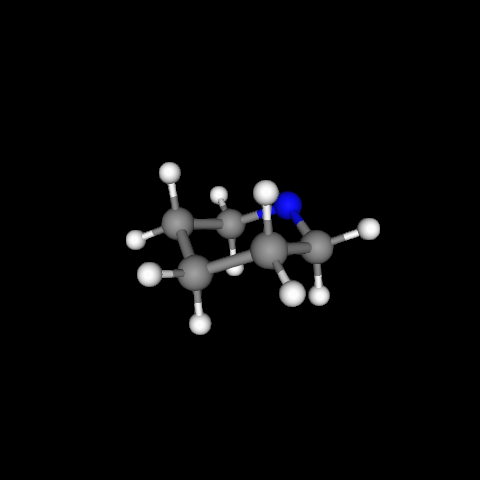
\includegraphics[width=0.5\textwidth]{Imagenes_QM/Ciclohexano3D.png}
    \caption{Conformación de silla en 3D (Ciclohexano).}
\end{figure}

Como se puede ver en la imagen, esa es la perspectiva desde la que se observa el anillo. 
Si aún no logras visualizarlo en 3D, no te preocupes: a mí me costó horas entenderla, 
pero te aseguro que es así. 

Aunque en esta imagen solo muestro el ciclohexano (con un solo \ce{O}), lo hago para que 
la imagen no se sature y se aprecie lo esencial: la geometría. Básicamente, la única 
diferencia con la glucosa es que donde aquí hay hidrógenos, en la glucosa hay grupos 
hidroxilo (\ce{-OH}).

\textbf{¿Por qué la celulosa forma fibras fuertes y el almidón no?}

La respuesta está en la silla. Si observas la imagen 3D, notarás que los enlaces 
salen en dos direcciones:
\begin{itemize}
    \item \textbf{Axial:} Hacia arriba o hacia abajo (recto).
    \item \textbf{Ecuatorial:} Hacia los lados (diagonal).
\end{itemize}

En la celulosa (enlace \(\beta(1\to4)\)), \textbf{todos} los grupos \ce{-OH} y los 
enlaces de la cadena están en posición ecuatorial (hacia los lados). Esto permite 
que las cadenas se empaqueten de forma lineal y recta, formando fibras muy 
resistentes e insolubles. En cambio, en el almidón (enlace \(\alpha\)), uno de los 
enlaces es axial, lo que obliga a la cadena a doblarse en forma de hélice. \\

\textbf{Reacción:}
\begin{reaccion}
    \schemestart
        \chemfig[cram width=2pt]{
        ?[1](-[:200]@{op1,.5}{O}-[:160])<[:-50](-[:170]HO)<[:10](-[:310]OH)>[:-10]
        (-[:20]O
        -[:-20](-[:60]?[2](-[:190]OH))<[:10](-[:210]-[:-60]OH)<[:-10]O>[:50](-[:-20]@{cl1,.5}{O}-[:20])-[:190]?[2](-[:60]OH))
        -[:130]O-[:190]?[1](-[:150]-[:60]OH)
        }
        \arrow{->[\ce{NaIO4}][\qty{40}{\celsius}]}[270, 1]
        \chemfig[cram width=2pt]{
        (-[:-10]-[:15]O-[:-50](=[:270,0.7]O)
        (-[:20]O
        -[:-20](-[:60](=[:90,0.7]O)(-[:190]OH))<[:10](-[:210]-[:-60]OH)<[:-10]O>[:50](-[:-20]@{cl2,.5}{O}-[:20])-[:190](=[:90]O))
        -[:130]O-[:190]?[1](-[:150]-[:60]OH)
        )(-[:200]@{op2,.5}{O}-[:160])<[:-50](-[:170]HO)<[:10](=[:270,0.7]O)
        }
        \arrow{->[\ce{NaBH4}][]}[270, 1]
        \chemfig[cram width=2pt]{
        (-[:-10]-[:15]O-[:-50](-[:270,0.7]OH)
        (-[:20]O
        -[:-20](-[:60](-[:90,0.7]OH)(-[:190]OH))<[:10](-[:210]-[:-60]OH)<[:-10]O>[:50](-[:-20]@{cl3,.5}{O}-[:20])-[:190](-[:90,0.7]OH))
        -[:130]O-[:190]?[1](-[:150]-[:60]OH)
        )(-[:200]@{op3,.5}{O}-[:160])<[:-50](-[:170]HO)<[:10](-[:270,0.7]OH)
        }
    \schemestop
    
    \polymerdelim[height=30pt, depth=30pt, indice=n]{op1}{cl1}
    \polymerdelim[height=30pt, depth=30pt, indice=n]{op2}{cl2}
    \polymerdelim[height=30pt, depth=30pt, indice=n]{op3}{cl3}
\end{reaccion}

\textbf{Solubilidad:}

Depende de los enlaces de hidrógeno y la polarizabilidad. En este ejemplo, 
aunque la celulosa no es soluble, va a tener una gran capacidad de retener 
líquidos (formar suspensiones en el agua). Es por eso que una hoja de papel 
no se disuelve, pero sí se empapa. \\


El PCC es un \textbf{agente oxidante suave}:

\begin{reaccion}
    \schemestart
        \chemfig{-[:30]-[:-30]OH}
        \arrow{->[PCC][DCM]}
        \chemfig{-[:30](=[:90]O)-[:-30]H}
        \arrow{-/>[\text{Se detiene aquí}]}[0,2]
        \chemfig{-[:30](=[:90]O)-[:-30]OH}
    \schemestop
\end{reaccion}

Hace la oxidación sin llegar a ácido carboxílico, por lo que la reacción se 
detiene en el aldehído.

\textbf{¿Qué es el PCC y DCM?}\\ 
PCC:

\begin{reaccion}
    \schemestart
        \chemfig{*6(=\chembelow{\charge{90:3pt=$\scriptstyle\color{catred}+$}{N}}{H}-=-=-)}
        \chemfig{Cr(=[:90]O)(=[:270]O)(-[:0]Cl)(-[:180]\charge{90:1pt=$\scriptstyle\color{anblue}-$}{O})}
    \schemestop
\end{reaccion}

DCM:
\begin{reaccion}
    \schemestart
        \chemname{\chemfig{C(-[:-25]H)(<:[:290]H)(-[:90]Cl)(<[:210]Cl)}}{Diclorometano \\ Cloruro de metileno}
    \schemestop
\end{reaccion}

El PCC es el agente y el diclorometano es el disolvente. Es importante especificar 
el disolvente en una reacción porque por ejemplo el \ce{KMnO4} o el \ce{Na2Cr2O7} 
ocupan agua para disolverse, si no evidentemente no se llevara a cabo la reacción 
o no de forma homogénea.

\textbf{Ésteres}

\begin{reaccion}
    \schemestart
        \chemname{\chemfig{-[:-30]O-[:30]\charge{270:5pt=$\scriptstyle\color{catred}+3$}{}(=[:90]O)-[:-30]-[:30]-[:-30]\charge{90:5pt=$\scriptstyle\color{catred}+3$}{}(=[:270]O)-[:30]O-[:-30]}}{Succinato de dimetilo}
        \arrow{->[\ce{LiAlH4}][THF]}
        \chemname{\chemfig{\charge{90:2pt=$\scriptstyle\color{anblue}-$}{O}-[:30]-[:-30]-[:30]-[:-30]-[:30]\charge{90:2pt=$\scriptstyle\color{anblue}-$}{O}}}{Intermediario}
        \arrow{->[\ce{H3O^{\color{catred}{+}}}][]}[270]
        \chemname{\chemfig{OH-[:30]\charge{90:2pt=$\scriptstyle\color{anblue}-1$}{}-[:-30]-[:30]-[:-30]\charge{270:2pt=$\scriptstyle\color{anblue}-1$}{}-[:30]OH}}{Butano Diol}
        \arrow{->[\ce{KMnO4}][]}[180]
        \chemname{\chemfig{OH-[:30]\charge{270:5pt=$\scriptstyle\color{catred}+3$}{}(=[:90]O)-[:-30]-[:30]-[:-30]\charge{90:5pt=$\scriptstyle\color{catred}+3$}{}(=[:270]O)-[:30]OH}}{Ácido succínico}
        \arrow{->[H2SO4][]}[270, 1.5]
        \chemname{\chemfig{
        @{op,.5}-[:30](=[:90]O)-[:-30]-[:30]-[:-30](=[:270]O)-[:30]O-[:-30]@{cl,.5}
        }}{Oligómero (cadena en crecimiento)}
    \schemestop
    \polymerdelim[height=25pt, depth=10pt, indice=crecimiento]{op}{cl}
\end{reaccion}

Lo interesante de todo esto es que el \textbf{succinato de dimetilo} se puede 
extraer de frutas verdes, por lo que teóricamente podríamos realizar esta síntesis 
a partir de guayaba o manzana verde.

No sé si lo notaron, pero además de lo obvio (en el primer paso, una reducción 
de un éster), pasaron muchas más cosas. 
Primero, rompimos el enlace \ce{C-O} y \ce{C=O} de los extremos para formar un 
alcohol primario. 
Después, volvimos a oxidar, pero ahora no formamos ésteres, formamos ácidos 
carboxílicos, que tienen el mismo n.o., pero como es obvio, no son iguales. 
Para al final hacer una esterificación de Fischer, que si nos damos cuenta, es 
la misma que habíamos hecho hace 2 clases. 
Como vimos, esta esterificación si se repite \(n\) veces puede generar un polímero, 
un poliéster. 
Qué loco, ¿no? Todo se va conectando, para que puedas desde manzana verde sacar 
el poliéster, más específicamente el PBS (poli(butilen succinato)) con el que 
podrías fabricar no sé... tu pantalón. \\

\textbf{Otra reacción de oxidación para llevar a ácidos carboxílicos:}

\begin{reaccion}
    \schemestart
        \chemname{\chemfig{*6((-\charge{90:3pt=$\scriptstyle\color{anblue}-3$}{C}H_3)=-=(-\charge{90:3pt=$\scriptstyle\color{anblue}-3$}{C}H_3)-=-)}}{\(p\)-xileno}
        \arrow{->[$\Delta$][\ce{KMnO4}, $-12\ce{e-}$]}[0, 1.8]
        \chemname{\chemfig{*6((-\charge{90:5pt=$\scriptstyle\color{catred}+3$}{}(=[:270]O)-[:150]OH)=-=(-\charge{270:5pt=$\scriptstyle\color{catred}+3$}{}(=[:90]O)-[:-30]OH)-=-)}}{Ácido tereftálico}
    \schemestop
\end{reaccion}

Es evidente que en este proceso fueron perdidos 12 electrones ($-12\ce{e-}$) por 
lo que hay varios intermediarios. Sin embargo, debido a que el agente oxidante es 
fuerte y se calienta, estos intermediarios prácticamente pasan súper rápido; 
además, no son de interés, por lo que los omito. 
Pero existen, fueron parte del proceso, solo que no son el foco de atención.

Misma pregunta que hace rato \textbf{¿Qué es el \ce{LiAlH4} y THF?} \\

\ce{LiAlH4}:
\begin{reaccion}
    \schemestart
        \chemname{\chemfig{Li^{\color{catred}{+}}}
        \charge{45:3pt=$\scriptstyle\color{anblue}-$}{\chemleft[\chemfig{Al(<:[:-25]H)(<[:290]H)(-[:90]H)(-[:210]H)}\chemright]}}
        {Hidruro de litio y aluminio}
    \schemestop
\end{reaccion}

THF:
\begin{reaccion}
    \schemestart
        \chemname{\chemfig{[:18]*5(---O--)}}{Tetrahidrofurano}
    \schemestop
\end{reaccion}

\phantomsection
\addcontentsline{toc}{subsubsection}{Clase 15 -- 15/10/2026: Reducción de nitrilos y alquinos}
\subsubsection*{\textcolor{blueunam}{Clase 15 -- 15/10/2026: Reducción de nitrilos y alquinos}}

\begin{itemize}
    \item Reducción de nitrilos para detener aldehídos o aminas
    \item Reducción de triples enlaces
\end{itemize}

Antes de comenzar, quiero aclarar un tipo de notación que es algo
contraintuitivo.

Nosotros sabemos que un triple enlace típicamente se puede ver así:
\begin{reaccion}
    \schemestart
        \chemfig{-[:30]-[:-30]~[:30]-[:-30]-[:30]}
    \schemestop
\end{reaccion}

Y sabemos que esto significa:
\begin{reaccion}
    \schemestart
        \chemfig{CH_3-[:30]CH_2-[:-30]C~[:30]C-[:-30]CH_2-[:30]CH_3}
    \schemestop
\end{reaccion}

Nada complicado y algo de toda la vida, pero a partir de aquí se emplean
notaciones algo contraintuitivas como lo son:
\begin{reaccion}
    \schemestart
        \chemfig{R-~N}
    \schemestop
\end{reaccion}

Que parece algo raro porque se ve como una línea mega larga; más bien
parece que el que lo escribió hizo la línea muy larga y solo puso el
triple enlace al final de ella. Sin embargo, esto realmente se traduce a:
\begin{reaccion}
    \schemestart
        \chemfig{R-C~N}
    \schemestop
\end{reaccion}

Esta notación suele pasar sobre todo donde no se pone explícitamente un
ángulo. Realmente la notación es la misma que la del primer ejemplo, pero
al no tener un ángulo, no se percibe claramente dónde está el carbono.

\textbf{Reducción de alquinos:}
La reducción de un alquino permite obtener alquenos con estereoquímica
controlada. El producto depende del agente reductor y de las condiciones.

\begin{reaccion}
\setchemfig{atom sep=1.6em}
\schemestart
\chemname{
    \chemfig{
        *6((-CH3O)-=-
            (-[:30]~[:30]-[:30]*6(-=-(-OCH3)=-=))
            =-=)
    }
}{1,2-bis(4-metoxifenil)etino}
\arrow(.mid east--.south west){->[\ce{Na}, \ce{NH3}(l)]}[45,2]
\chemname{
    \chemfig{
        *6((-CH3O)-=-
            (-[:30]=[:-30]-[:30]*6(-=-(-OCH3)=-=))
            =-=)
    }
}{(\textit{E})-1,2-bis(4-metoxifenil)eteno\\
\small(\textit{trans})}
\arrow(@c1.mid east--.north west){->[\ce{H2}, Lindlar]}[-45,2]
\chemname{
    \chemfig{
        *6((-CH3O)-=-
            (-[:30]=[:0]-[:-30]*6(-=-(-OCH3)=-=))
            =-=)
    }
}{(\textit{Z})-1,2-bis(4-metoxifenil)eteno\\
\small(\textit{cis})}
\schemestop
\chemnameinit{}
\end{reaccion}

Para este caso, con sodio en amoniaco líquido la reducción da el alqueno
\textit{trans}. Con hidrógeno sobre catalizador de Lindlar da el isómero
\textit{cis}. En ambos casos el triple enlace se reduce a doble y el
esqueleto carbonado se conserva.

\begin{notaimportante}
\textbf{E/Z.}
En cada carbono del doble enlace se asigna por prioridad CIP: gana el
sustituyente de mayor número atómico unido directamente. Si los dos
ganadores quedan en lados opuestos, es \textit{E}; si quedan del mismo
lado, es \textit{Z}. Aquí \textit{E} = \textit{trans} y \textit{Z} =
\textit{cis}, porque cada carbono lleva un H y un arilo. La asignación
detallada se cubre en la clase de nomenclatura.
\end{notaimportante}

De las dos rutas de reducción selectiva, la siguiente que se detalla es
la del catalizador de Lindlar, que da una configuración cis:

\textbf{Envenenamiento de catalizador:} inactivar ciertas posiciones del
catalizador para que no reaccionen. En el Lindlar, parte de los sitios de
paladio se envenenan con acetato de plomo(II), Pb(OAc)$_2$. Los sitios
activos restantes reducen el alquino a alqueno, pero no alcanzan a seguir
hasta alcano.

\begin{center}
\begin{tikzpicture}[scale=1,>=Stealth,remember picture]
    \fill[gray!25] (-3.6,-0.5) rectangle (3.6,0);
    \draw[thick] (-3.6,-0.5) rectangle (3.6,0);
    \node[below] at (0,-0.7) {\small \ce{CaCO3}};

    \foreach \x in {-3,-2.25,-1.5,-0.75,0,0.75,1.5,2.25,3} {
        \filldraw[fill=gray!70] (\x,0.25) circle (0.18);
    }
    \foreach \x in {-2.25,-0.75,1.5,2.25} {
        \fill (\x,0.25) circle (0.18);
    }

    \foreach \x in {-3,-1.5,0,0.75,3} {
        \draw[thick] (\x,0.43) -- (\x,0.85) node[above] {\small H};
    }

    \coordinate (PdA) at (-1.5, 0.43);
    \coordinate (PdB) at (0.75, 0.43);

    \node at (0,3.8) {%
        \chemfig[atom sep=2.5em]{%
            [:-30]*6((-CH3O)-=-
                (-[:0]@{Cl}C~[:0]@{Cr}C-[:0]*6(-=-(-OCH3)=-=))
                =-=)
        }%
    };

    \filldraw[fill=gray!70] (-3.2,-2.6) circle (0.15);
    \node[right] at (-3.0,-2.6) {\small Pd activo};
    \fill (0.8,-2.6) circle (0.15);
    \node[right] at (1.0,-2.6) {\small Pd envenenado};
\end{tikzpicture}
\chemmove{
    \draw[dashed, ->, gray, shorten <=2pt, shorten >=2pt] (PdA)
        .. controls +(90:1.2) and +(270:1.2) .. (Cl);
    \draw[dashed, ->, gray, shorten <=2pt, shorten >=2pt] (PdB)
        .. controls +(90:1.2) and +(270:1.2) .. (Cr);
}
\end{center}

\begin{reaccion}
    \schemestart
    \arrow{->[\ce{H2}, Lindlar]}[270,1]
        \chemfig{
        *6(-=(-[:-30](-[:225]H)=[:0](-[:-45]H)-[:30]*6(-=-(-OCH3)=-=))
        -
        =-(-CH3O)=)
    }
    \schemestop
\end{reaccion}

\textbf{Por qué el producto es cis.} El alquino se adsorbe sobre la
superficie de Pd: los electrones $\pi$ del triple enlace se coordinan a
los sitios metálicos activos, y por eso la molécula queda tendida sobre
la placa con un solo lado expuesto hacia arriba. El \ce{H2} también se
adsorbe y se disocia en átomos de H sobre la misma superficie. Cuando los
dos H se transfieren al triple enlace, ambos vienen del mismo lado de la
molécula; no hay forma de que uno llegue por encima del plano molecular y
el otro por debajo, porque el alquino está apoyado sobre la placa. La
adición es syn por construcción del sistema heterogéneo, y el doble
enlace queda con los dos H del mismo lado y los dos arilos del otro. Eso
es el isómero cis.

\textbf{Por qué no sigue hasta alcano.} Tiene dos motivos combinados.
Primero, el alqueno recién formado se adsorbe con menos fuerza que el
alquino, así que tiende a desorberse y abandonar la superficie antes de
que llegue un segundo par de H. Segundo, el veneno reduce el número de
sitios activos: con menos sitios disponibles, y además fragmentados en
zonas aisladas, la probabilidad de que el alqueno encuentre dos H sobre
sitios adyacentes cae mucho. El alqueno se va antes de que ocurra la
segunda hidrogenación, y el producto se detiene ahí.

\textbf{Relación con el envenenamiento.} Si no hubiera veneno, el alqueno
seguiría adsorbido y terminaría como alcano. El veneno no cambia el
mecanismo ni la estereoquímica: solo reduce la actividad de la superficie
lo suficiente para que la reacción se detenga en la primera etapa. Por
eso el Lindlar da cis y no trans ni alcano. \\

\textbf{Ahora se detallará la reacción para la ruta trans.}

\textbf{Reducción con metales disueltos (\ce{Na}/\ce{NH3}).}
El segundo camino para reducir un alquino no usa superficie catalítica,
sino electrones libres en disolución. El sodio metálico cede su único
electrón de valencia y el amoniaco líquido actúa como fuente de protones.
El resultado neto es una \textit{anti}-adición de hidrógeno: los dos H
terminan en caras opuestas del doble enlace, y el alqueno final es
\textit{trans}.

\textbf{Mecanismo en cuatro etapas.}
(1)~El primer electrón del \ce{Na} entra al $\pi^*$ del alquino y forma un
radical anión. (2)~El \ce{NH3} protona el carbono que quedó con exceso de
carga negativa, generando un radical vinílico. (3)~El segundo electrón
del \ce{Na} entra al SOMO del radical y forma un anión vinílico.
(4)~Una segunda protonación completa la reducción y libera el alqueno.

\setchemfig{atom sep=1.5em}
\begin{reaccion}
\schemestart
% Paso 1: alquino + 1er SET
\chemfig{
    [:-30]*6((-CH3O)-=-
        (-[:0]@{Cl1}-[:0]@{Cr1}-[:0]*6(-=-(-OCH3)=-=))
        =-=)
}
\chemmove{
    \orbital[pos={(Cl1)}, scale=0.4, pcolor=blue!60, ncolor=red!60]{pz}
    \orbital[pos={(Cr1)}, scale=0.4, pcolor=blue!60, ncolor=red!60]{pz}
    \shade[ball color=blue!60] ($(Cl1)+(0,0.15)$) circle (1pt);
    \shade[ball color=blue!60] ($(Cr1)+(0,0.15)$) circle (1pt);
    \node[circle, draw, thick, fill=gray!20, inner sep=1pt, font=\scriptsize]
        (Na1) at ($(Cl1)+(-1.5,1.2)$) {Na};
    \shade[ball color=orange!80] ($(Na1)+(0.25,0)$) circle (1.2pt);
    \draw[->, thick, orange!80, shorten <=1pt, shorten >=1pt]
        (Na1.south east) to[bend left=25] ($(Cl1)+(0,0.35)$);
    \node[above, orange!80, font=\scriptsize]
        at ($(Na1)+(0.5,0.3)$) {e$^-$};
}
\arrow{->}[0,1.2]
% Paso 2: radical anion (enlace de orden fraccionario)
\chemfig{
    [:-30]*6((-CH3O)-=-
        (-[:0]@{Cl2}-[:0,,,,ddbond={-}]@{Cr2}-[:0]*6(-=-(-OCH3)=-=))
        =-=)
}
\chemmove{
    \orbital[pos={(Cl2)}, scale=0.4, pcolor=blue!60, ncolor=red!60]{pz}
    \orbital[pos={(Cr2)}, scale=0.4, pcolor=red!60, ncolor=blue!60]{pz}
    \shade[ball color=blue!60] ($(Cl2)+(0,0.12)$) circle (1pt);
    \shade[ball color=blue!60] ($(Cl2)+(0,0.28)$) circle (1pt);
    \shade[ball color=red!60] ($(Cr2)+(0,0.20)$) circle (1pt);
    \node[font=\scriptsize, text=blue!80] at ($(Cl2)+(-0.3,-0.4)$) {$\ominus$};
}
\arrow{->[\ce{NH3}]}[270,1.2]
% Paso 3: geometria trans (ya se ve el doblez)
\chemfig{
    [:-30]*6((-CH3O)-=-
        (-[:30](-[:90]H)=[:-30]@{Cr3}-[:30]*6(-=-(-OCH3)=-=))
        =-=)
}
\chemmove{
    \orbital[pos={(Cr3)}, scale=0.4, pcolor=red!60, ncolor=blue!60]{pz}
    \shade[ball color=red!60] ($(Cr3)+(0,0.20)$) circle (1pt);
    \node[circle, draw, thick, fill=gray!20, inner sep=1pt, font=\scriptsize]
        (Na2) at ($(Cr3)+(1.2,1.8)$) {Na};
    \shade[ball color=orange!80] ($(Na2)+(-0.25,0)$) circle (1.2pt);
    \draw[->, thick, orange!80, shorten <=1pt, shorten >=1pt]
        (Na2.south west) to[bend right=25] ($(Cr3)+(0,0.35)$);
    \node[above, orange!80, font=\scriptsize]
        at ($(Na2)+(-0.5,0.3)$) {e$^-$};
}
\arrow{->}[180,1.2]
% Paso 4: anion vinilico (sigue trans)
\chemfig{
    [:-30]*6((-CH3O)-=-
        (-[:30](-[:90]H)=[:-30]@{Cr4}-[:30]*6(-=-(-OCH3)=-=))
        =-=)
}
\chemmove{
    \orbital[pos={(Cr4)}, scale=0.4, pcolor=red!60, ncolor=blue!60]{pz}
    \shade[ball color=red!60] ($(Cr4)+(0,0.12)$) circle (1pt);
    \shade[ball color=red!60] ($(Cr4)+(0,0.28)$) circle (1pt);
    \node[font=\scriptsize, text=blue!80] at ($(Cr4)+(0.3,-0.4)$) {$\ominus$};
}
\arrow{->[\ce{NH3}]}[270,1.2]
% Paso 5: alqueno trans final
\chemfig{
    [:-30]*6((-CH3O)-=-
        (-[:30](-[:90]H)=[:-30](-[:270]H)-[:30]*6(-=-(-OCH3)=-=))
        =-=)
}
\schemestop
\end{reaccion}

\textbf{Por qué el producto es trans.}
Un triple enlace es rígido porque su orden de enlace es 3: los dos
carbonos no pueden girar uno respecto al otro sin romperlo. Un doble
enlace tampoco gira, porque su orden es 2. Pero el radical anión no está
en ninguno de esos dos extremos: reparte tres electrones entre el orbital
enlazante y el antienlazante, y su orden de enlace queda cerca de 1.5.
Ese valor intermedio significa que el enlace C--C está a medio aflojar:
suficientemente rígido para mantener la molécula unida, suficientemente
flojo para permitir que los carbonos giren uno respecto al otro.
(La figura lo dibuja con un trazo sólido y otro punteado para representar
ese orden fraccionario, ni triple ni doble.) Aprovechando esa libertad,
la molécula busca la posición más cómoda: los dos anillos aromáticos son
voluminosos y se repelen, así que se acomodan en lados opuestos. Esa
posición es la \textit{trans}. Cuando entra el primer H (etapa~2), el
orden de enlace sube a 2, el doble enlace queda completo y la molécula se
congela en la geometría que ya tenía. Las etapas~3 y~4 solo terminan la
reducción; la geometría se decidió antes.

\textbf{Contraste con el Lindlar.}
El Lindlar da \textit{cis} porque los dos H vienen de la misma superficie
(adición \textit{syn} forzada geométricamente). Los metales disueltos dan
\textit{trans} porque el intermedio radical anión puede rotar antes de
que la segunda mitad de la reacción se complete (adición \textit{anti}).
Son dos mecanismos distintos: heterogéneo contra homogéneo por
transferencia electrónica.